\documentclass[UTF8]{beamer}
\usepackage{ctex}

\usetheme{Madrid}
\usefonttheme[onlymath]{serif}
%\usecolortheme{}
\usepackage{tikz}
\usepackage{graphicx}
\usepackage{subfigure}
\usepackage{amsmath}
\usepackage{braket}

\usepackage{algorithm,algorithmic}

\bibliographystyle{plain}
%information
\title{Husimi图}
\author{BHL}

\begin{document}
\frame{\titlepage}
\begin{frame}\frametitle{目录}
    \tableofcontents
\end{frame}
%----------------------------------------------------------%
%
\section{论文中基本概念的梳理}
\begin{frame}\frametitle{目录}
    \tableofcontents[currentsection]
\end{frame}
\subsection{流算符}
\begin{frame}\frametitle{流算符}
    在量子力学的课本中,在某一点的概率流算符(the probability flux)算符可以定义为
    \begin{equation}
        \hat{\mathbf{j}}_{\mathbf{r}} = \frac{1}{2m}(\ket{\mathbf{r}}\bra{\mathbf{r}}\hat{\mathbf{p}}+\hat{\mathbf{p}}\ket{\mathbf{r}}\bra{\mathbf{r}})
        \label{flux:def}
    \end{equation}
    其中$\mathbf{r}$和$\mathbf{p}$分别是质量为$m$的粒子的位置和动量。

    同时,可以计算出概率流算符的平均值
    \begin{equation}
        \begin{aligned}
            \bra{\psi}\hat{\mathbf{j}}_{\mathbf{r}}\ket{\psi} & =
            \frac{\mathrm{i}\hbar}{2m}(
            \mathrm{\psi}(\mathbf{r})\nabla\mathrm{\psi}^{*}(\mathbf{r})
            -\mathrm{\psi}^{*}(\mathbf{r})\nabla\mathrm{\psi}(\mathbf{r})
            )                                                                                                                                                   \\
                                                              & =\frac{1}{m}\Im[\mathrm{\psi}^{*}(\mathbf{r})(-\mathrm{i}\hbar\nabla)\mathrm{\psi}(\mathbf{r})] \\
                                                              & =\frac{1}{m}\Im[\mathrm{\psi}^{*}(\mathbf{r})\hat{\mathbf{p}}\mathrm{\psi}(\mathbf{r})]
            \label{flux:ave}
        \end{aligned}
    \end{equation}
\end{frame}
\begin{frame}\frametitle{流算符的“矛盾”}
    从式(\ref{flux:ave})可以看出流算符的概念有一些“矛盾”,我们知道位置很精确的同时,还需要一些关于动量的信息。\\
    \begin{block}{原文\cite{mason2013quantum}}
        The concept of “flux at a point” seems paradoxical because we say something about momentum while also knowing position precisely.
    \end{block}
\end{frame}
\begin{frame}\frametitle{造成“矛盾”的原因}
    \begin{block}{Heisenberg不确定性原理}
        \Large
        \begin{center}
            $\Delta x \, \Delta p \geqslant \frac{\hbar}{2}$
        \end{center}
    \end{block}
\end{frame}
%
\begin{frame}\frametitle{流算符}
    对于传统的流算符,存在如下问题:
    \begin{itemize}
        \item 概率流是否可以被测量
        \item 具有时间反演对称性的系统,其概率流会消失。
    \end{itemize}
\end{frame}
%-------------------------------------------------------------%
\subsection{流算符的本征态}
\begin{frame}
    高斯型基矢可以写为
    \begin{equation}
        \braket{\mathbf{r}|\mathbf{r}_0,\sigma}=N_{_\sigma}^{d/2}\mathrm{e}^{-\frac{(\mathbf{r}-\mathbf{r}_{_0})^2}{4\sigma^2}}
    \end{equation}
    其中$N_{_\sigma}^{d/2} = (\sigma\sqrt{2\pi})^{-1}$,将式(\ref{flux:def})改写成
    \begin{equation}
        \hat{\mathbf{j}}_{\mathbf{r}_0,\sigma} = \frac{1}{2m}(\ket{\mathbf{r}_0,\sigma}\bra{\mathbf{r}_0,\sigma}\hat{\mathbf{p}}+\hat{\mathbf{p}}\ket{\mathbf{r}_0,\sigma}\bra{\mathbf{r}_0,\sigma})
        \label{flux:sigma}
    \end{equation}
\end{frame}
\begin{frame}\frametitle{流算符的本征态}
    写出本征方程:
    \begin{equation}
        \hat{\mathbf{j}}_{\mathbf{r}_0,\sigma,i}\,\ket{\lambda_{\sigma,i}}=\lambda_{\sigma,i}\ket{\lambda_{\sigma,i}}
        \label{flux:eigeq}
    \end{equation}
    式(\ref{flux:sigma})与(\ref{flux:eigeq})中的$i$是空间的维度指标。
    该本征方程的解可以写为
    \begin{equation*}
        \ket{\lambda_{\sigma,i}}=\ket{\mathbf{r}_0,\sigma}+a\hat{p}_i\ket{\mathbf{r}_0,\sigma}
    \end{equation*}
    可以将求解本征方程转换成:
    \begin{equation}
        \hat{\mathbf{j}}_{\mathbf{r}_0,\sigma}\ket{\lambda_{\sigma,i}} =
        \frac{1}{2m}(a\braket{\hat{p}_i^2}_{\sigma}\ket{\mathbf{r}_0,\sigma}+\hat{p}_i\ket{\mathbf{r}_0,\sigma})
    \end{equation}
\end{frame}
\begin{frame}\frametitle{流算符的本征态}
    由于$\braket{\hat{p}_i^2}_{\sigma}=\frac{\hbar^2}{4\sigma^2}$因此有两个本征值可写为
    \begin{equation}
        \lambda_{\sigma,i,\pm}=\pm\frac{\hbar}{4m\sigma}
    \end{equation}
    本征态在坐标表象的形式如下
    \begin{equation}
        \braket{\mathbf{r}|\lambda_{\sigma,i,\pm}}=
        \braket{\mathbf{r}|\mathbf{r}_0,\sigma}\pm
        \frac{\mathrm{i}}{\sigma}\mathbf{e}_i\cdot(\mathbf{r}-\mathbf{r}_0)\braket{\mathbf{r}|\mathbf{r}_0,\sigma}
        \label{husimi:eigstate}
    \end{equation}
\end{frame}
\begin{frame}
    \frametitle{谐振子的本征态}
    \begin{align}
        \braket{\mathbf{r}|0} & =\braket{\mathbf{r}|\mathbf{r}_0,\sigma}\nonumber                                                 \\
        \braket{\mathbf{r}|1} & =\frac{\mathrm{e}_i\cdot(\mathbf{r}-\mathbf{r}_0)}{\sigma}\braket{\mathbf{r}|\mathbf{r}_0,\sigma} \\
        \vdots \nonumber
    \end{align}
\end{frame}
\begin{frame}
    \frametitle{流算符和本征态的矩阵表示}
    流算符:
    \begin{equation*}
        \hat{j}_{\mathbf{r}_0,\sigma,i}=
        \begin{bmatrix}
            0                  & +\mathrm{i}\lambda & 0\cdots & 0      \\
            -\mathrm{i}\lambda & 0                  & 0\cdots & 0      \\
            0                  & 0                  & 0\cdots & 0      \\
            \vdots             & \vdots             & \ddots  & \vdots \\
            0                  & 0                  & \cdots  & 0
        \end{bmatrix}
    \end{equation*}
    本征态:
    \begin{equation*}
        \,\ket{\lambda_{1}}=
        \begin{bmatrix}
            1           \\
            -\mathrm{i} \\
            0           \\
            \vdots
        \end{bmatrix}
        \,\ket{\lambda_{2}}=
        \begin{bmatrix}
            1          \\
            \mathrm{i} \\
            0          \\
            \vdots
        \end{bmatrix}
        \,\ket{\lambda_{3}}=
        \begin{bmatrix}
            0 \\
            0 \\
            1 \\
            \vdots
        \end{bmatrix}
        \cdots
    \end{equation*}
\end{frame}
\begin{frame}
    \frametitle{拓展后的流算符}
    利用基矢的完备性,可以将流算符写成
    \begin{align}
        \bra{\psi}\hat{j}_{\mathbf{r}_0,\sigma,i}\ket{\psi} & =\sum_{i=1}^\infty
        \bra{\psi}\hat{j}_{\mathbf{r}_0,\sigma,i}\ket{\lambda_i}\braket{\lambda_i|\psi}                                                                                                                                       \\
                                                            & =\lambda | \braket{\psi|\lambda_1}|^2-\lambda|\braket{\psi|\lambda_2}|^2                                                                                        \\
                                                            & =\frac{\mathrm{i}\hbar}{4m\sigma^2}[\bra{\psi}\mathbf{e}_i\cdot(\mathbf{r}-\mathbf{r}_0)\ket{\mathbf{r}_0,\sigma}\braket{\psi|\mathbf{r}_0,\sigma}^{*}\nonumber
        \\&-\bra{\psi}\mathbf{e}_i\cdot(\mathbf{r}-\mathbf{r}_0)\ket{\mathbf{r}_0,\sigma}^{*}\braket{\psi|\mathbf{r}_0,\sigma}]
    \end{align}
    其中$\lambda=\frac{\hbar}{4m\sigma}$课本上定义的流(式(\ref{flux:ave}))可以看作是$\sigma\rightarrow0^{+}$的特殊情况。
\end{frame}
%------------------------------------------------------------%
%
\section{Husimi表象}
\begin{frame}\frametitle{目录}
    \tableofcontents[currentsection]
\end{frame}
%-----------------------------------------------------------%
\subsection{流算符的测量}
\begin{frame}
    \frametitle{流算符的测量}
    将式(\ref{husimi:eigstate})与下面的泰勒展开进行比较
    \begin{equation}
        \mathrm{e}^{\pm\frac{\mathrm{i}}{\sigma}\mathbf{e}_i\cdot(\mathbf{r}-\mathbf{r}_0)}\approx 1\pm
        \frac{\mathrm{i}}{\sigma}\mathbf{e}_i\cdot(\mathbf{r}-\mathbf{r}_0)
    \end{equation}
    将流算符的本征态和相干态联系起来,可以定义
    \begin{equation}
        \braket{\mathbf{r}|\mathbf{r}_0,\mathbf{k}_0,\sigma}=
        N_{_\sigma}^{d/2}\mathrm{e}^{-\frac{(\mathbf{r}-\mathbf{r}_{_0})^2}{4\sigma^2}+\mathrm{i}\mathbf{k}_{_0}\cdot\mathbf{r}}
    \end{equation}
    \begin{block}{条件}
        \Large
        \begin{equation*}
            \sigma\,k \ll 1
        \end{equation*}
    \end{block}
\end{frame}
\begin{frame}
    \frametitle{相干态中的不确定关系$\sigma$}
    \begin{equation}
        \Delta x \,\propto\, 1/\Delta k \,\propto\, \sigma
    \end{equation}
    \begin{block}{}
        对于$\sigma \rightarrow 0$的情况:动量空间的$\sigma_k=\infty$,实空间的$\sigma_r=0$,与传统的流算符的测量结果相同。
    \end{block}
\end{frame}
\begin{frame}
    \frametitle{相空间分布函数}
    \begin{itemize}
        \item Wigner准概率分布函数
        \item Husimi分布函数(相空间的概率密度)
    \end{itemize}
\end{frame}
\begin{frame}
    \frametitle{Husimi函数}
    将$\ket{\psi}$与流算符的本征态$\ket{\mathbf{r}_0,\mathbf{k}_0,\sigma}$作内积可得
    \begin{align}
        \braket{\mathbf{\psi}|\mathbf{r}_0,\mathbf{k}_0,\sigma} & = \int \,\mathrm{d}\mathbf{r}\braket{\mathbf{\psi}|\mathbf{r}}\braket{\mathbf{r}|\lambda,\mathbf{k}_0,\sigma}                                                          \\
                                                                & = \int \,\mathrm{d}\mathbf{r}\ \psi^{*}(\mathbf{r})\,N_{\sigma}^{d/2}\mathrm{e}^{-\frac{(\mathbf{r}-\mathbf{r}_0)^2}{4\sigma^2}+\mathrm{i}\mathbf{k}_0\cdot\mathbf{r}}
        \label{husimi:psiproj}
    \end{align}
    利用式(\ref{husimi:psiproj}),应用相干态定义一种波函数的测量值(测试波包):
    \begin{equation}
        \mathrm{Hu}(\mathbf{r}_0,\mathbf{k}_0, \sigma,\psi(\mathbf{r}))=\left\lvert\Braket{\mathbf{\psi}|\mathbf{r}_0,\mathbf{k}_0,\sigma}\right\rvert^2
        \label{husimi:function}
    \end{equation}
\end{frame}
\begin{frame}
    \frametitle{Husimi矢量}
    Husimi矢量:通过加权每一个用于测试的$\mathbf{k}_0$。
    \begin{equation*}
        \mathrm{Hu}(\mathbf{r}_0,\mathbf{k}_0, \sigma,\psi(\mathbf{r}))= \left\lvert \int \,\psi^{*}(\mathbf{r})\,N_{_\sigma}^{d/2}\mathrm{e}^{-\frac{(\mathbf{r}-\mathbf{r}_{_0})^2}{4\sigma^2}+\mathrm{i}\mathbf{k}_{_0}\cdot\mathbf{r}} \,\mathrm{d}\mathbf{r} \right\rvert^2
    \end{equation*}
    \begin{figure}
        \centering
        \subfigure[加权前$\mathbf{k}_0$]{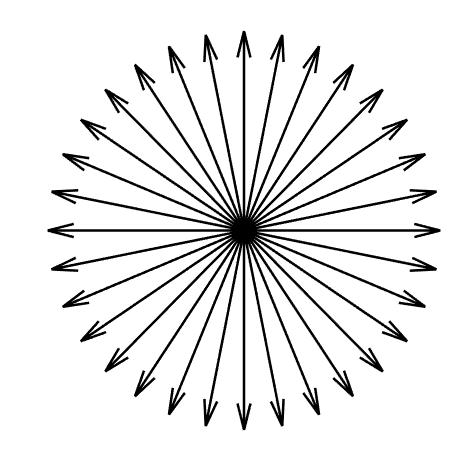
\includegraphics[width=0.4\textwidth]{../images/figure/arrow.png}}
        \subfigure[加权后$\mathbf{k}_0$]{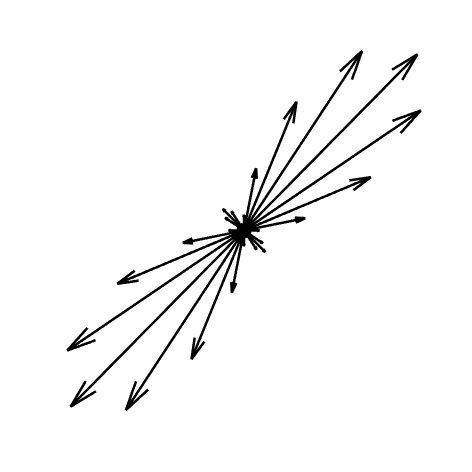
\includegraphics[width=0.4\textwidth]{../images/figure/processed_arrow.png}}
    \end{figure}
\end{frame}
\begin{frame}
    \frametitle{Husimi矢量}
    \begin{center}
        \begin{tikzpicture}
            \draw[->] (-5.5,0) -- (5.5,0)node[right]{$x$};
            \draw[->] (0,-1.5) -- (0,4.5)node[right]{$y$};
            \draw[domain=1:4.5, red, thick]
            plot(\x,{4*2.71828^(-(\x-1)^2)});
            \draw[domain=-4.5:1, red, thick]
            plot(\x,{4*2.71828^(-(\x-1)^2)});
            \draw[domain=-5:0, blue, thick]
            plot(\x,{cos((\x*100)});
            \draw[domain=0:5, blue, thick]
            plot(\x,{cos((\x*100)});
            \node[above right, rounded corners] at (3,4) {红色:$\braket{\mathbf{r}|\mathbf{r}_0,\mathbf{k}_0,\sigma}$};
            \node[above right, rounded corners] at (3,3) {蓝色:$\braket{\mathbf{r}|\psi}$};
        \end{tikzpicture}
    \end{center}
    只有在以$r_{_0}$为圆心,半径$r\approx 3\sqrt{2}\sigma$的圆内的点,才对Husimi函数值有贡献。
\end{frame}
%----------------------MMA---------------------------------%
\subsection{多模态分析算法}
\begin{frame}
    \frametitle{多模态分析算法}
    D. J. Mason在文中\cite{mason2012extending}\cite{mason2013quantum}关于Multi-Modal Analysis (MMA)算法的描述如下所示
    \begin{figure}
        \centering
        \includegraphics[width=0.5\textwidth]{./fig/MMA.png}
    \end{figure}
\end{frame}
\begin{frame}
    \frametitle{多模态分析算法}
    \begin{algorithm}[H]
        \caption{多模态分析法(MAA:Multi-Modal Analysis)}
        \label{alg:maa}
        \begin{algorithmic}[1]
            \STATE 用M个波矢\{$\mathbf{k}^{test}_{i}$\}生成测试平面波$\psi=\mathrm{e}^{\mathrm{i}\mathbf{k}_i^{test}\cdot\mathbf{r}}$ ,将每个测试平面波用N个测试波矢\{$\mathbf{k}_j$\}(非测试平面波的波矢)生成模板集合的成员。
            两组波矢\{$\mathbf{k}_{i}^{test}\}$和$\{\mathbf{k}_{j}\}$都位于色散等值线上。每个模板(个数为M)存储的值为$\mathbf{u}_i$,$\mathbf{u}_i$的每一个成员对应于Husimi函数(式\ref{husimi:function})值;
            \label{alg:maastep:create}
            \STATE 相似程度的衡量标准由$\mathbf{d}_i=\mathbf{v}\cdot\mathbf{u}_i$给出,其中矢量$\mathbf{v}$表示Husimi矢量,$\mathbf{u}_i$表示在步骤\ref{alg:maastep:create})中的每个模板;
            \STATE 找出集合\{$d_i$\}的极大值和对应的波矢$\mathbf{k}^{test}_i$,并将它们保存下来;
            \STATE 带波矢$\mathbf{k}^{test}_{i}$的轨迹的贡献由重新加权的矢量决定$\mathbf{u}_{i}\frac{d_{i}}{\mathbf{u}_{i}\cdot\mathbf{u}_{i}}$;
            \STATE Husimi矢量减去加权后的模板矢量,即$\mathbf{v}_{i}\rightarrow\mathbf{v}_{i}-\mathbf{u}_{i}\frac{d_{i}}{\mathbf{u}_{i}\cdot\mathbf{u}_{i}}$
            \STATE 将$\mathbf{v}$的所有负元素设为零;
            \label {alg:maastep:loopend}
            \STATE 重复步骤\ref{alg:maastep:create})\,-\,\ref{alg:maastep:loopend})直到$\mathbf{d}_{i}$低于一个阈值;
            \STATE 矢量集合\{$d_{i}\,\mathbf{k}^{test}_i$\}近似为处理后的Husimi流;
        \end{algorithmic}
    \end{algorithm}
\end{frame}

\begin{frame}[allowframebreaks]
    \frametitle{\textbf{MMA}的思想}
    将测试平面波与未知波的Husimi函数值进行比较,找到相似之处。
    \begin{figure}
        \centering
        \subfigure[$\psi^{test}=\mathrm{e}^{\mathrm{i}\mathbf{k}_{i}^{test}\cdot\mathbf{r}}$]
        {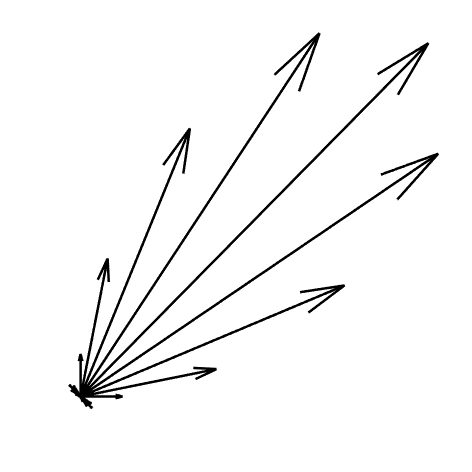
\includegraphics[width=0.42\textwidth]{../images/figure/PsiTest.png}}
        \qquad
        \subfigure[$\psi=\alpha\cos{(\mathrm{i}\mathbf{k}_1\cdot\mathbf{r})}+\beta\cos{(\mathrm{i}\mathbf{k}_2\cdot\mathbf{r})}$]
        {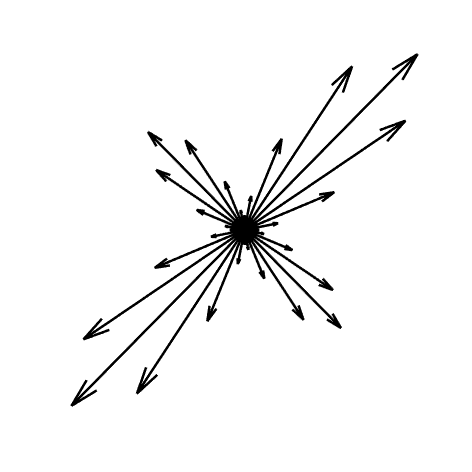
\includegraphics[width=0.42\textwidth]{../images/figure/PsiC.png}}
    \end{figure}
    \begin{columns}
        \begin{column}{0.62\textwidth}
            \begin{center}
                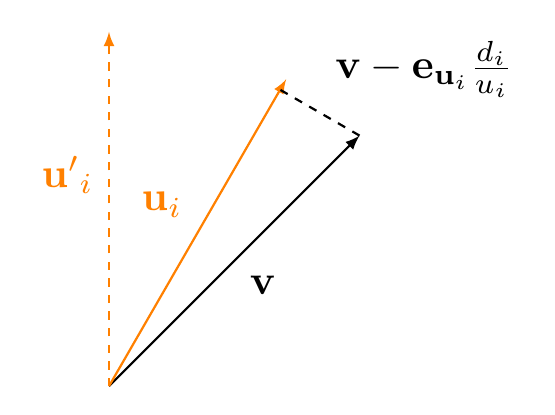
\begin{tikzpicture}[thick]
                    \coordinate (O) at (0,0);
                    \draw[-latex] (O) --node[below right, scale=1.5] {$\mathbf{v}$} (45:4.5);
                    \draw[-latex, orange] (O) --node[above left, scale=1.5] {$\mathbf{u}_i$} (60:4.5);

                    \draw[dashed] (45:4.5) --node[above right, scale=1.5] {$\mathbf{v}-\mathbf{e}_{\mathbf{u}_{i}}\frac{d_i}{u_i}$} (60:4.3466);
                    \draw[-latex, orange, dashed] (O) --node[above left, scale=1.5] {$\mathbf{u'}_i$} (90:4.5);
                    %垂线%
                \end{tikzpicture}
            \end{center}
        \end{column}
        \begin{column}{0.3\textwidth}
            {\normalsize 寻找$d_i$最大值}
            \Large
            \begin{equation*}
                d_i = \mathbf{v}\cdot\mathbf{u}_i
            \end{equation*}
            {\normalsize 其中$|\mathbf{v}| = 1,|\mathbf{u}_i| = 1$}
        \end{column}
    \end{columns}
\end{frame}

\begin{frame}[allowframebreaks]
    \frametitle{MMA的实际操作}
    \begin{figure}
        \centering
        \subfigure[处理前$\mathbf{v}$]{
            \includegraphics[width=0.36\textwidth]{fig/v.png}
        }
        $\stackrel{d_i=\mathbf{v}\cdot\mathbf{u}_i\text{卷积}}{\implies}$
        \subfigure[\{$d_i$\}]{
            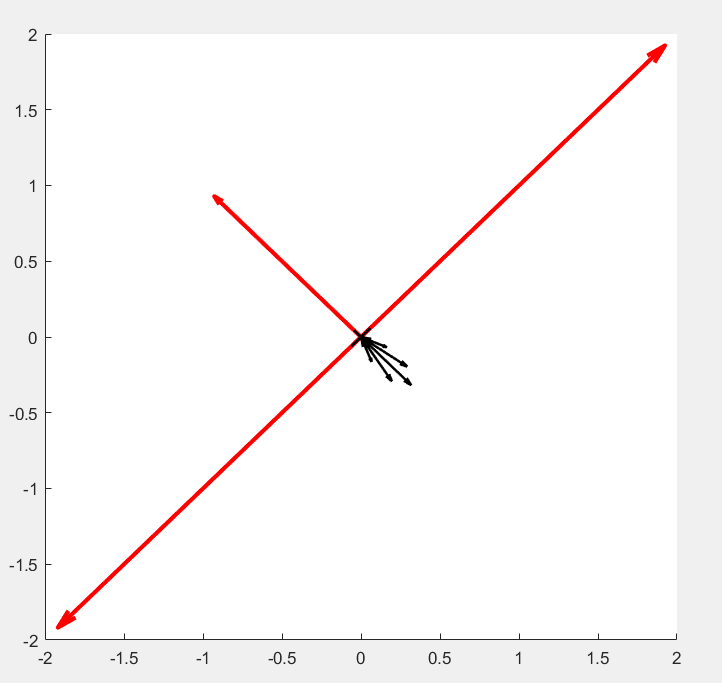
\includegraphics[width=0.42\textwidth]{fig/d.png}
        }
        $\stackrel{\max d_i}{\implies}$
        \subfigure[$\max d_i$对于的$u_i$]{
            \includegraphics[width=0.35\textwidth]{fig/u.png}
        }
        $\stackrel{\mathbf{v}\rightarrow\mathbf{v}-\mathbf{u}_{i}\frac{d_{i}}{\mathbf{u}_{i}\cdot\mathbf{u}_{i}}}{\implies}$
        \subfigure[处理后的$\mathbf{v}$和加权后的$\mathbf{u_{i_max}}$]{
            \includegraphics[width=0.35\textwidth]{fig/interaction.png}
        }
    \end{figure}
\end{frame}

\begin{frame}[allowframebreaks]
    \frametitle{\textbf{MMA}的流程}
    \begin{enumerate}
        \item 准备
              \begin{itemize}
                  \item 每个模板$\mathbf{u}_i=[u_i^1\ u_i^1\ \cdots u_i^N]$,其中每个成员$u_i^j=\mathrm{Hu}(\psi^{test},\mathbf{k}_j)$
                  \item Husimi矢量$\mathbf{v}=[v^1\ v^1\ \cdots v^N]$,其中每个成员$v^j=\mathrm{Hu}(\psi,\mathbf{k}_j)$
              \end{itemize}
        \item 寻找
              \begin{itemize}
                  \item $d_i = \mathbf{v}\cdot\mathbf{u}_i$
                  \item find $\ \max \{d_i\}$
                  \item $\max\{d_i\},\ \mathbf{k}_i^{test}$保存
              \end{itemize}
        \item $\mathbf{v}\rightarrow\mathbf{v}-\mathbf{u}_i\frac{d_i}{\mathbf{u}_i\cdot\mathbf{u}_i}$
        \item 将$\mathbf{v}$中小于零的值设为零
        \item 重复1)\,-\,6) 直到$d_i<eps$
        \item $\{d_i\mathbf{k}_i^{test}\}$就是Husimi流
    \end{enumerate}
\end{frame}

%-------------------------------------------------------------%
%
%-------------------------------------------------------------%
\section{复现的结果}
\begin{frame}\frametitle{目录}
    \tableofcontents[currentsection]
\end{frame}
\subsection{未处理的Husimi图}

\begin{frame}
    \frametitle{文中\cite{mason2013quantum}的图2}
    \begin{figure}
        \centering
        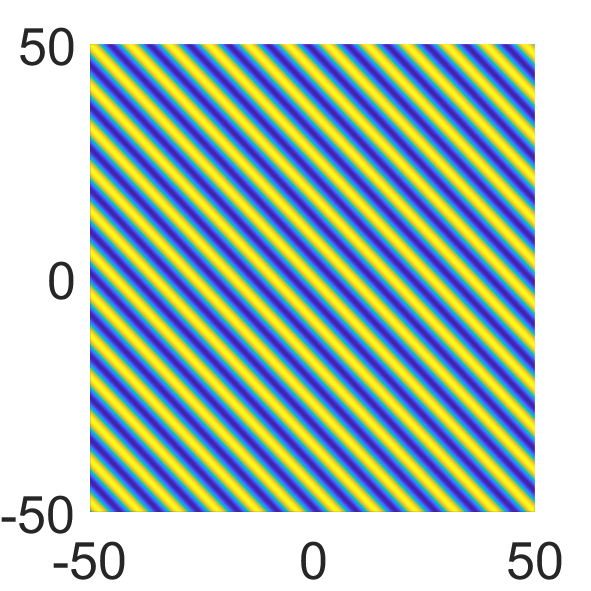
\includegraphics[width = 0.2\textwidth]{../images/figure/PsiA2.png}
        \quad
        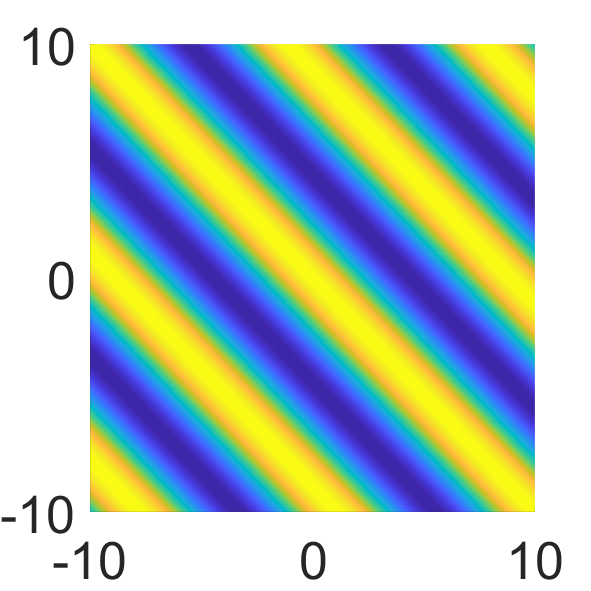
\includegraphics[width = 0.2\textwidth]{../images/figure/PsiA10.png}
        \quad
        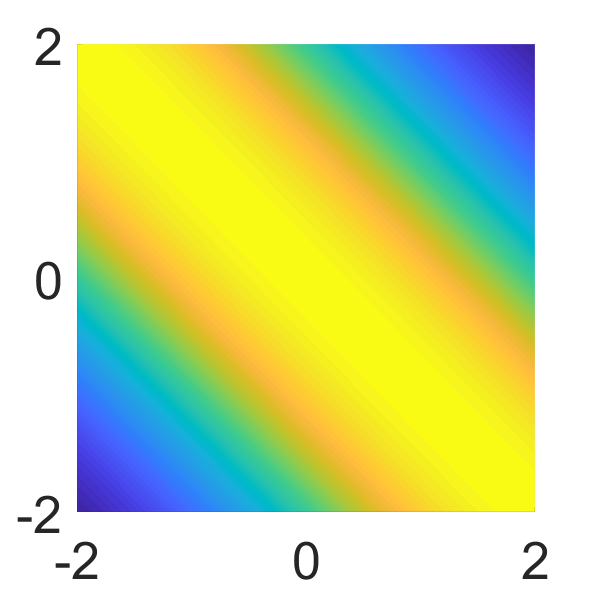
\includegraphics[width = 0.2\textwidth]{../images/figure/PsiA50.png}
        \quad
        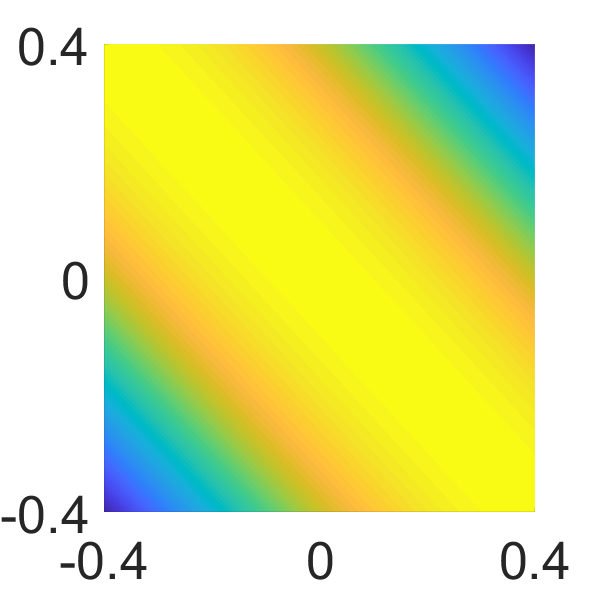
\includegraphics[width = 0.2\textwidth]{../images/figure/PsiA250.png}
        \subfigure[$ 2\% $]{
            \centering
            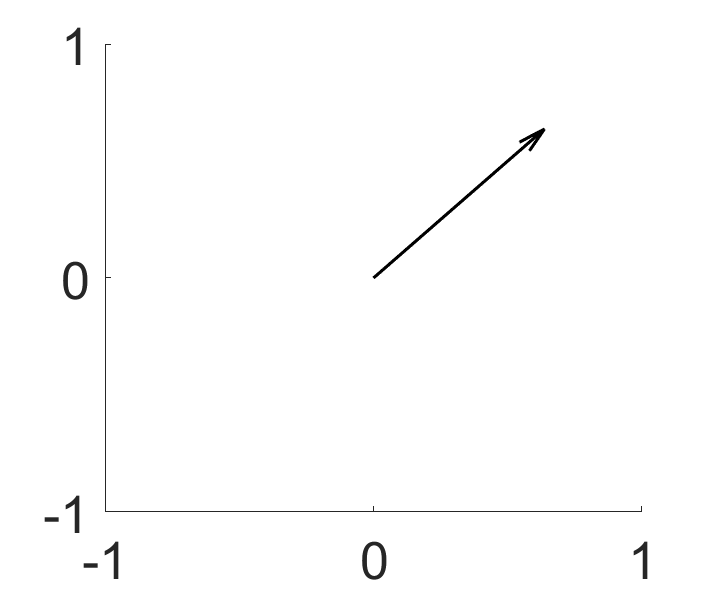
\includegraphics[width = 0.2\textwidth]{../images/figure/HuA2.png}
        }
        \subfigure[$ 10\% $]{
            \centering
            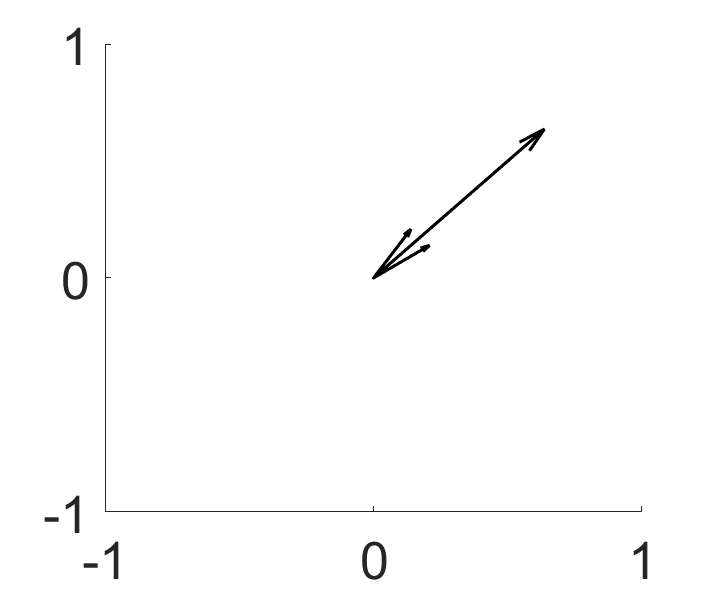
\includegraphics[width = 0.2\textwidth]{../images/figure/HuA10.png}
        }
        \subfigure[$ 50\% $]{
            \centering
            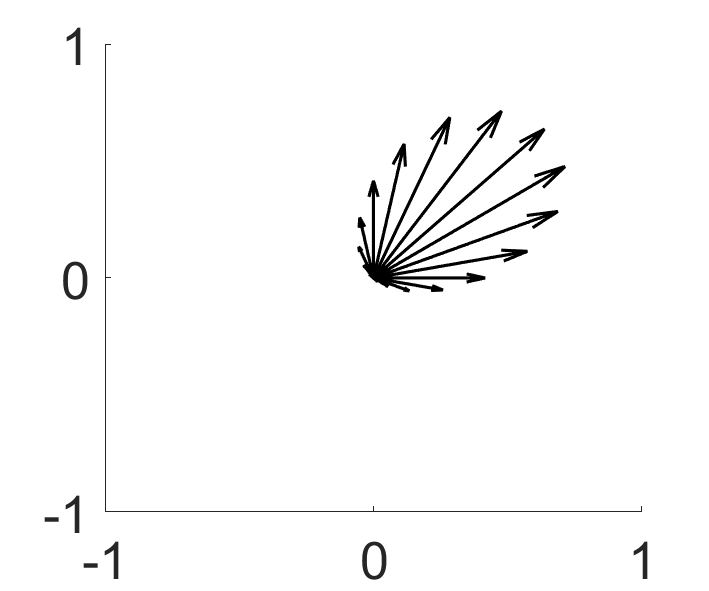
\includegraphics[width = 0.2\textwidth]{../images/figure/HuA50.png}
        }
        \subfigure[$ 250\% $]{
            \centering
            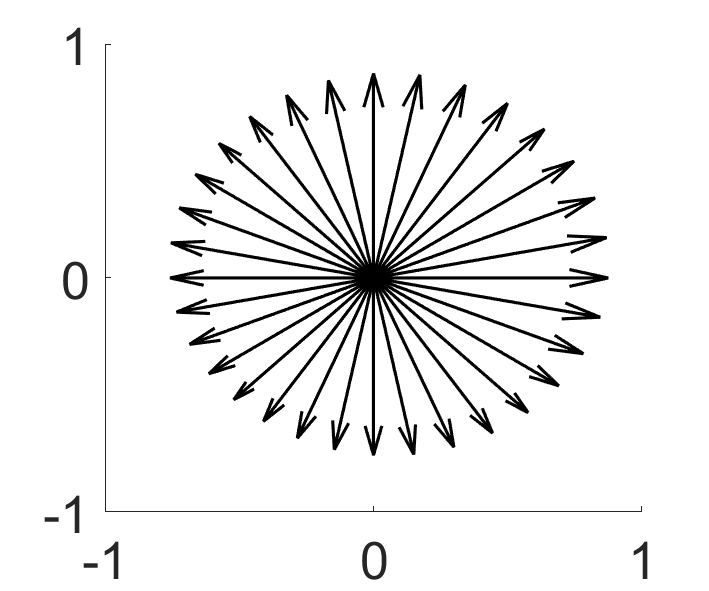
\includegraphics[width = 0.2\textwidth]{../images/figure/HuA250.png}
        }
        \caption{$\psi_A(\mathbf{r})=\mathrm{e}^{\mathrm{i}\mathbf{k}\cdot\mathbf{r}}$,小图$\Delta k/k$}
    \end{figure}
\end{frame}
\begin{frame}
    \frametitle{文中\cite{mason2013quantum}的图2}
    \begin{figure}
        \centering
        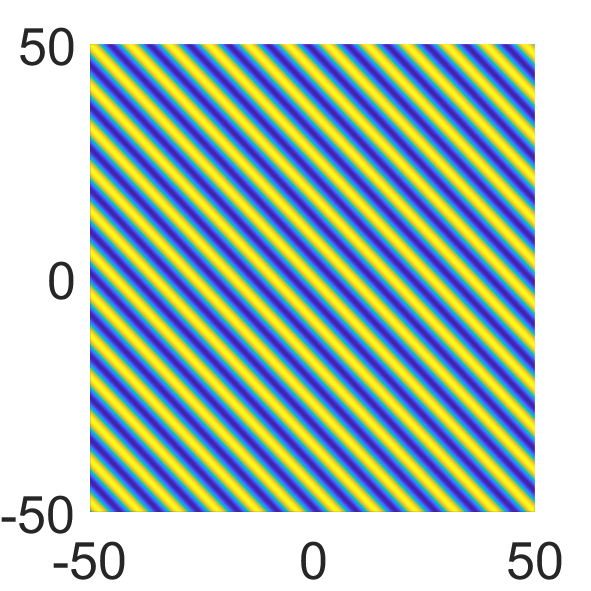
\includegraphics[width = 0.2\textwidth]{../images/figure/PsiB2.png}
        \quad
        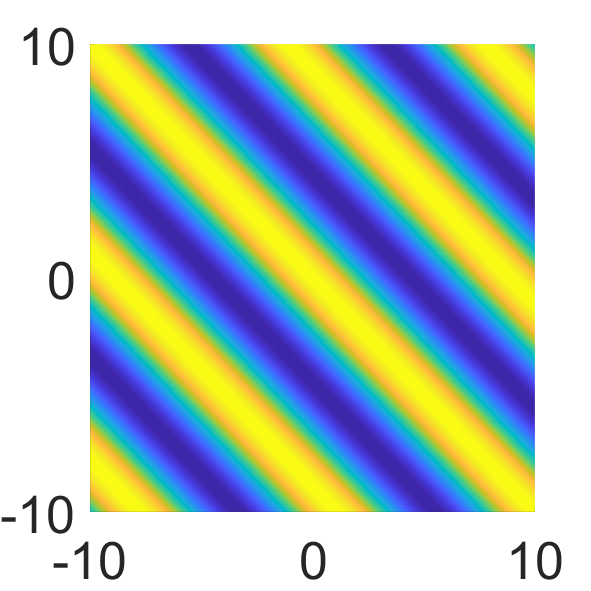
\includegraphics[width = 0.2\textwidth]{../images/figure/PsiB10.png}
        \quad
        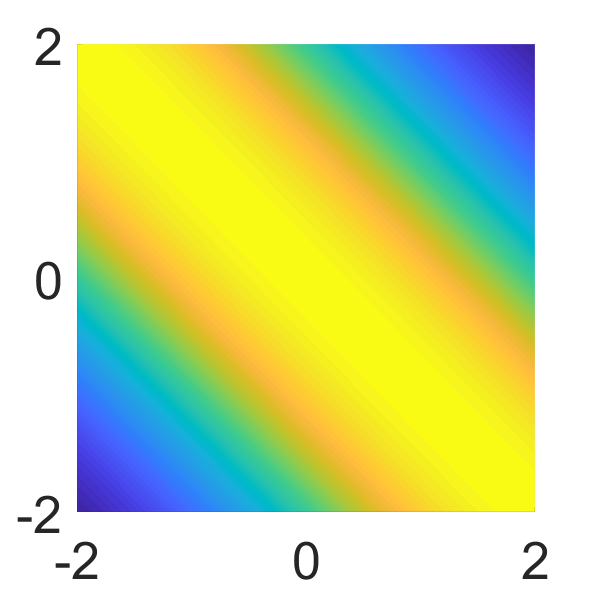
\includegraphics[width = 0.2\textwidth]{../images/figure/PsiB50.png}
        \quad
        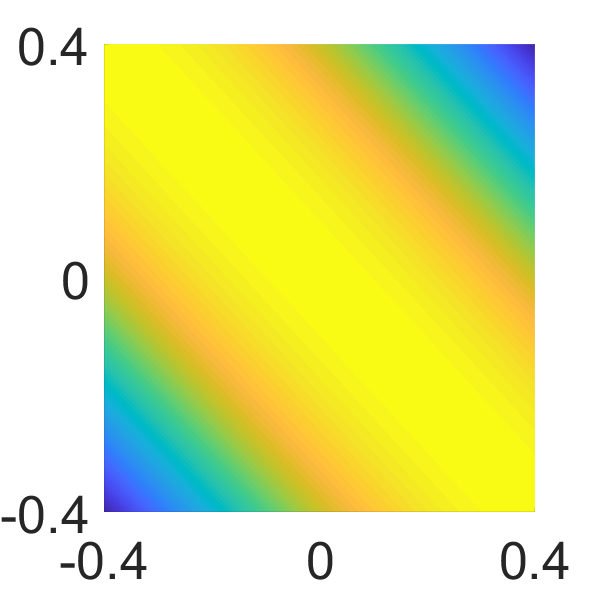
\includegraphics[width = 0.2\textwidth]{../images/figure/PsiB250.png}
        \subfigure[$ 2\% $]{
            \centering
            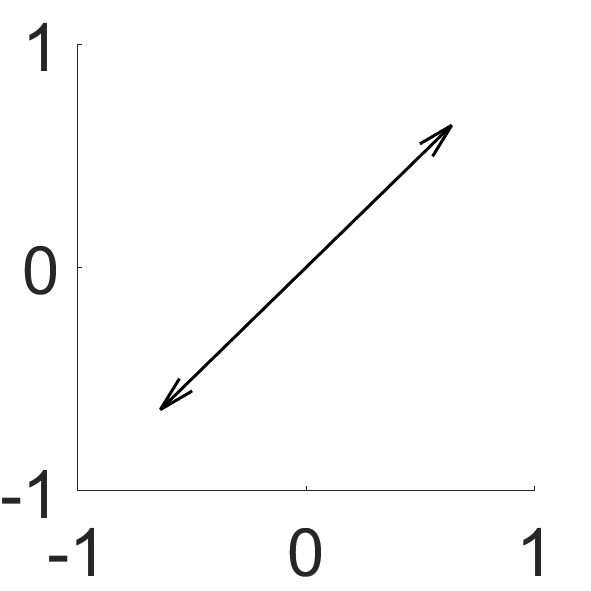
\includegraphics[width = 0.2\textwidth]{../images/figure/HuB2.png}
        }
        \subfigure[$ 10\% $]{
            \centering
            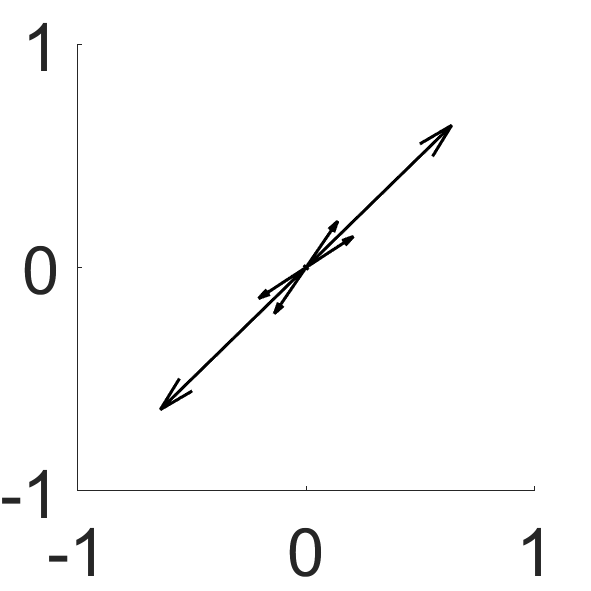
\includegraphics[width = 0.2\textwidth]{../images/figure/HuB10.png}
        }
        \subfigure[$ 50\% $]{
            \centering
            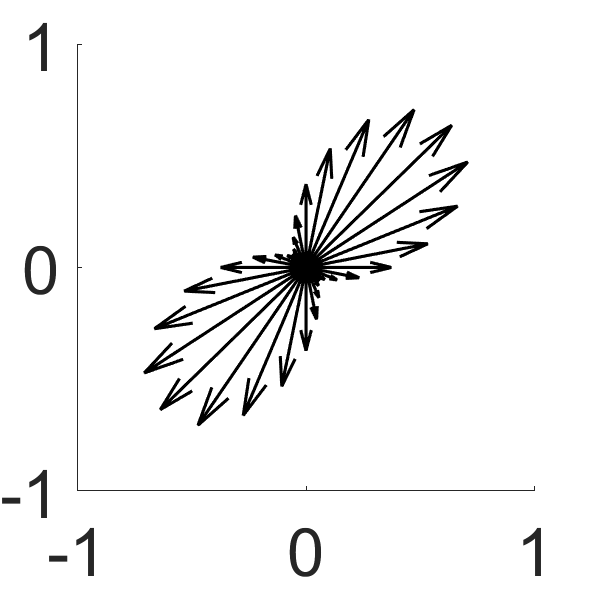
\includegraphics[width = 0.2\textwidth]{../images/figure/HuB50.png}
        }
        \subfigure[$ 250\% $]{
            \centering
            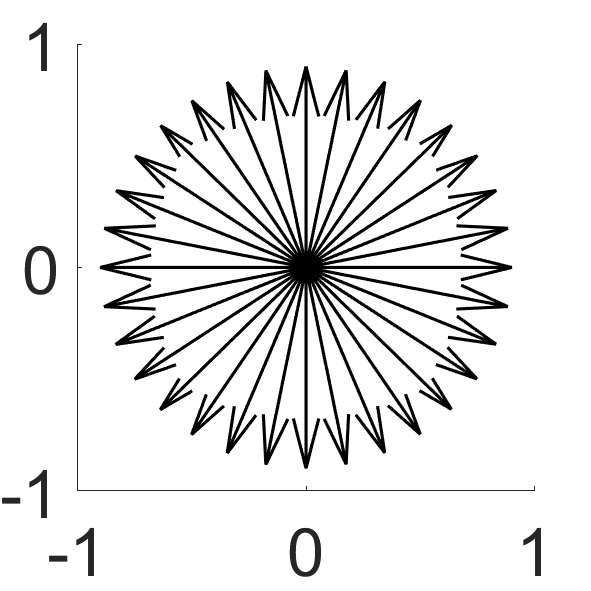
\includegraphics[width = 0.2\textwidth]{../images/figure/HuB250.png}
        }
        \caption{$\psi_B(\mathbf{r})=\cos (\mathbf{k}\cdot\mathbf{r}$,小图$\Delta k/k$}
    \end{figure}
\end{frame}
\begin{frame}
    \frametitle{文中\cite{mason2013quantum}的图3}
    \begin{figure}[h]
        \centering
        \subfigure[$ \Delta k /k = 30\%$ 时的Husimi图]
        {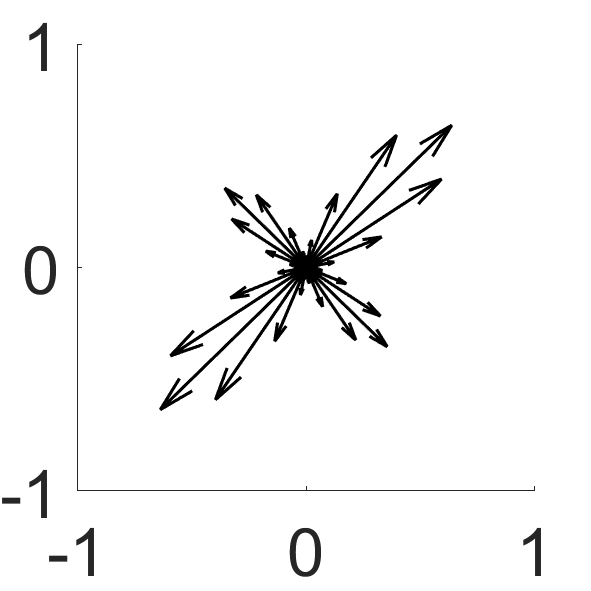
\includegraphics[width = 0.42\textwidth]{../images/figure/HuC30.png}}
        \qquad
        \subfigure[$ \Psi_C = \alpha\cos ({\mathrm{i}\mathbf{k}\cdot\mathbf{r}}) + \beta\cos ({\mathrm{i}\mathbf{k}\cdot\mathbf{r}})$]
        {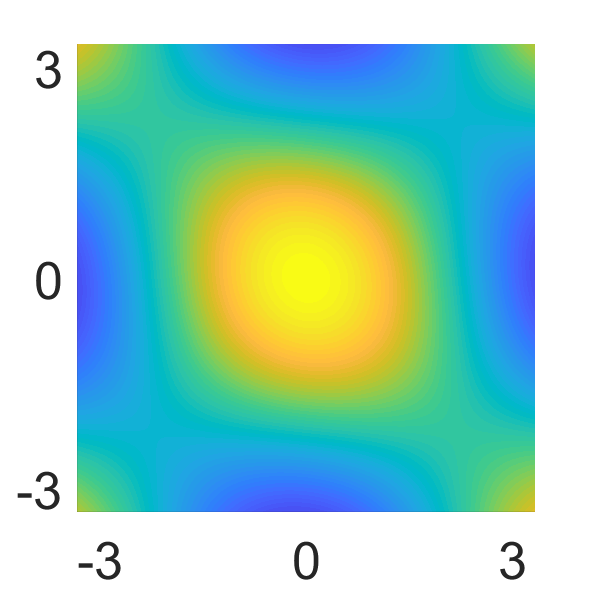
\includegraphics[width = 0.42\textwidth]{../images/figure/PsiC30.png}}
        \caption{Husimi图}
    \end{figure}
\end{frame}
%
%--------------------------------------------------------------%
\subsection{处理过的Husimi图}
\begin{frame}
    \frametitle{利用MMA算法处理过的$\psi_c$}
    \begin{figure}
        \centering
        \subfigure[]{
            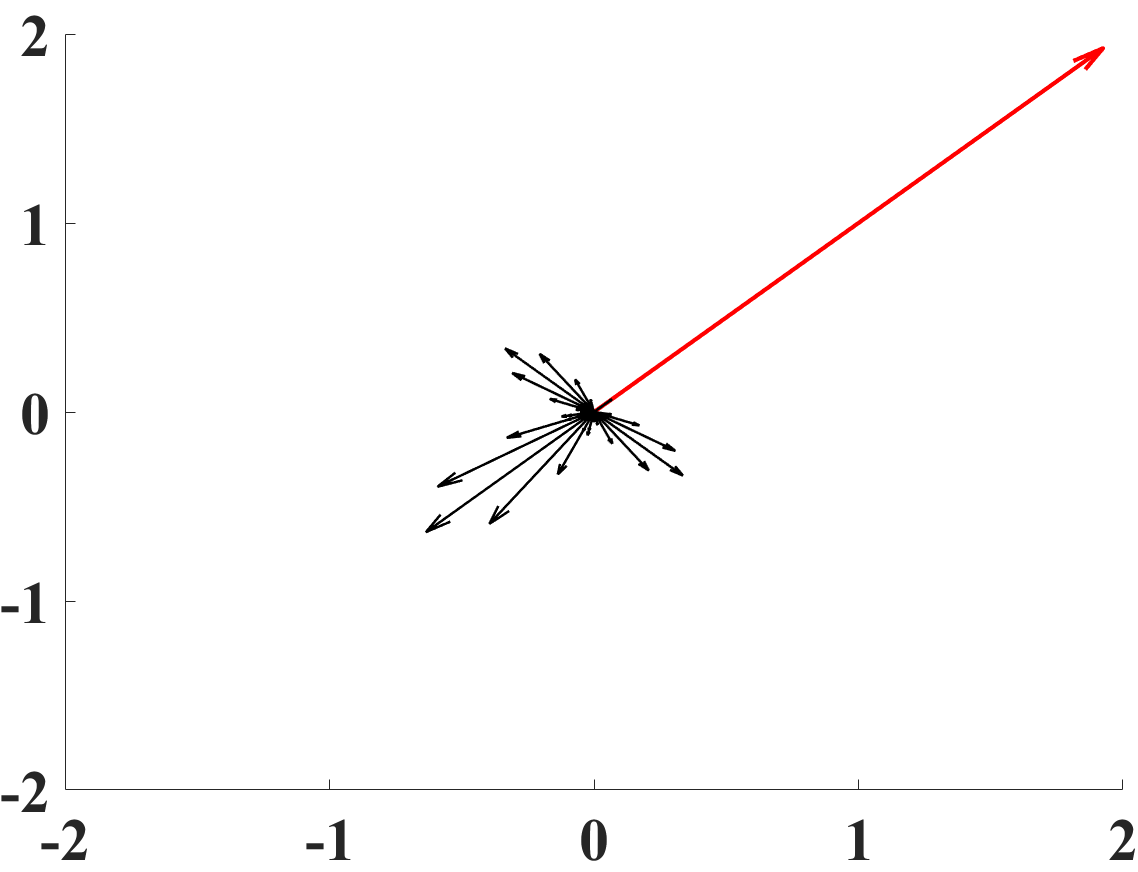
\includegraphics[width = 0.28\textwidth]{../images/figure/b.png}
        }
        \subfigure[]{
            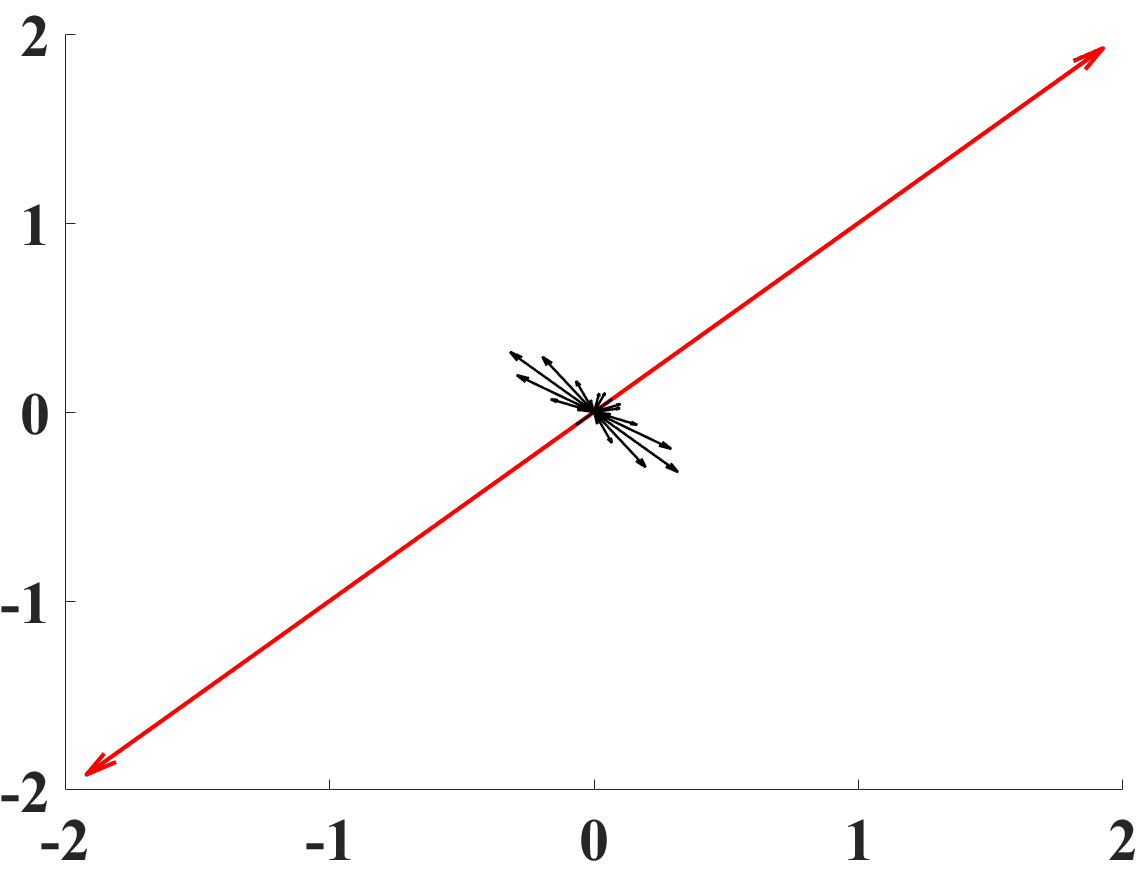
\includegraphics[width = 0.28\textwidth]{../images/figure/c.png}
        }\\
        \subfigure[]{
            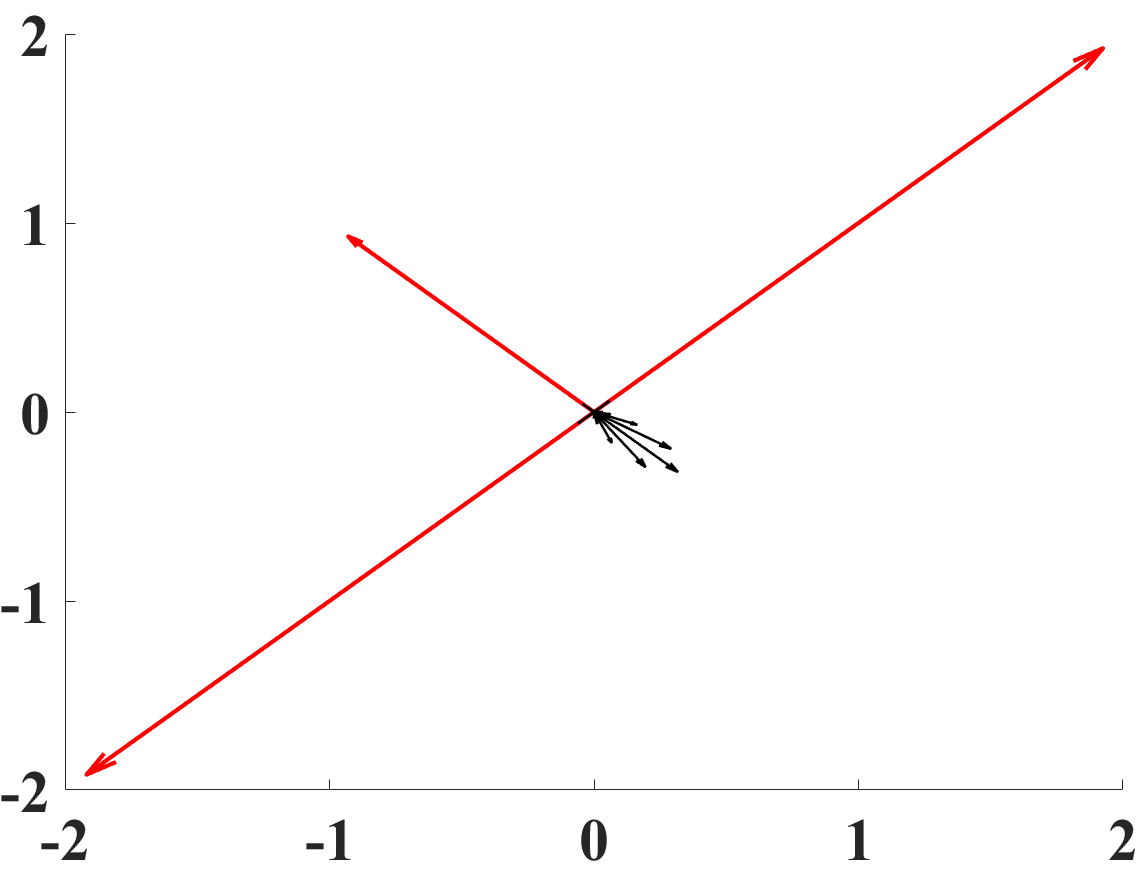
\includegraphics[width = 0.28\textwidth]{../images/figure/d.png}
        }
        \subfigure[]{
            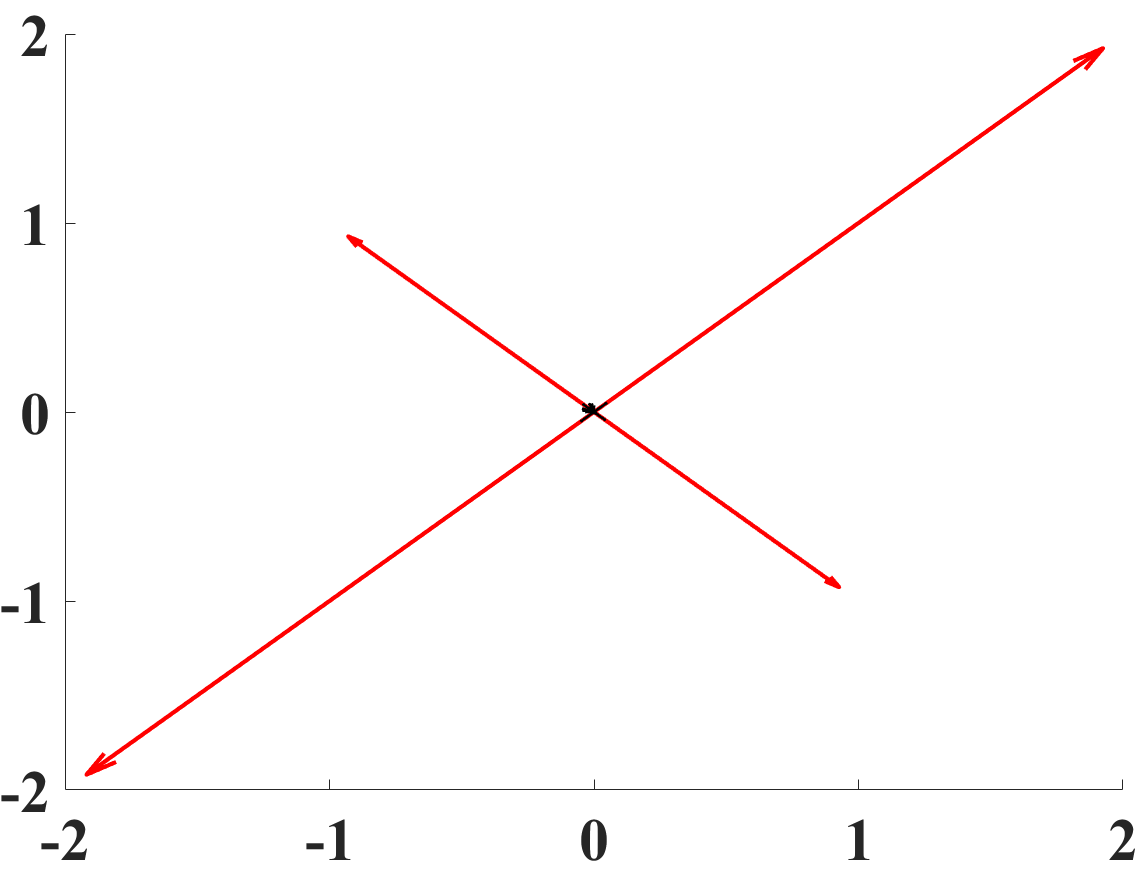
\includegraphics[width = 0.28\textwidth]{../images/figure/e.png}
        }
    \end{figure}
\end{frame}

% ---------------------------Circular system--------------------------------

\section{应用}
\begin{frame}\frametitle{目录}
    \tableofcontents[currentsection]
\end{frame}
\subsection{圆形系统}
\begin{frame}
    \frametitle{采样点}
    \begin{figure}
        \centering
        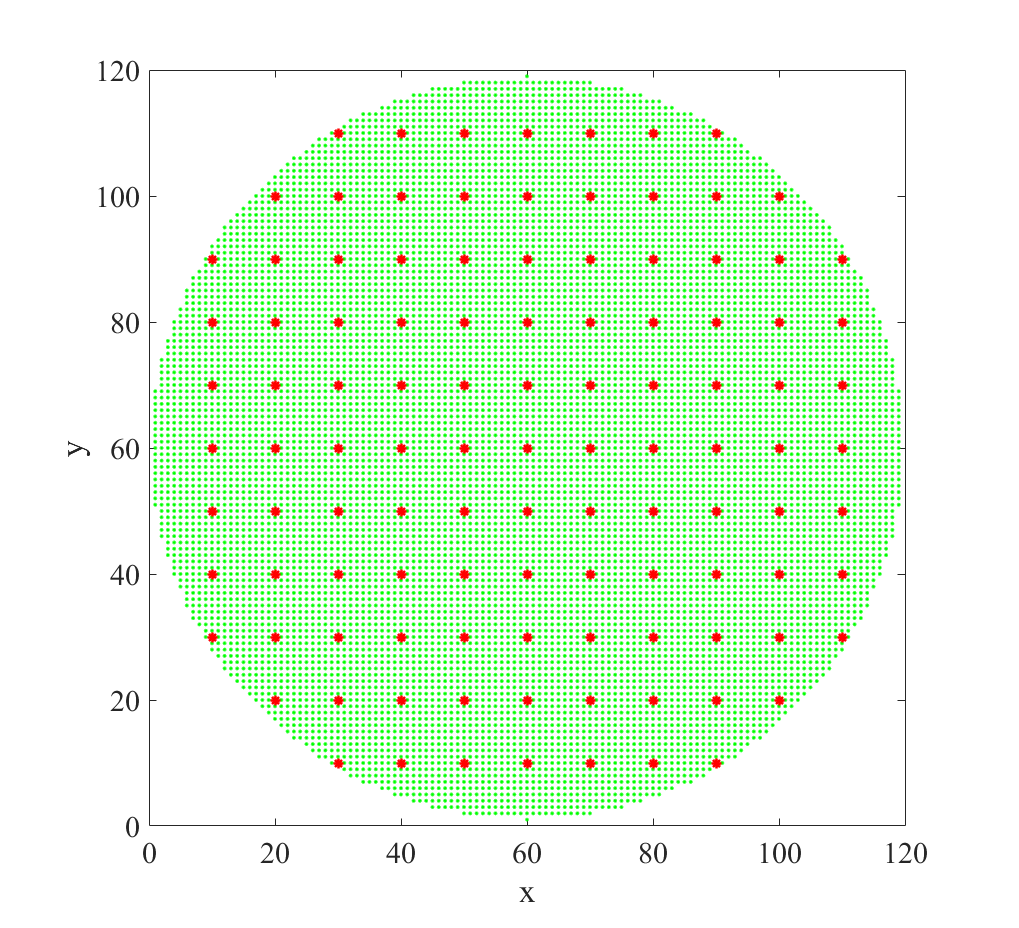
\includegraphics[width = 0.5\textwidth]{../images/figure/0.1_Mesh.png}
        \caption{红色:采样点;绿色:离散的格点}
    \end{figure}
\end{frame}

\begin{frame}
    \frametitle{硬墙}
    \begin{figure}
        \centering
        \subfigure[$n=91(m=0)$]{
            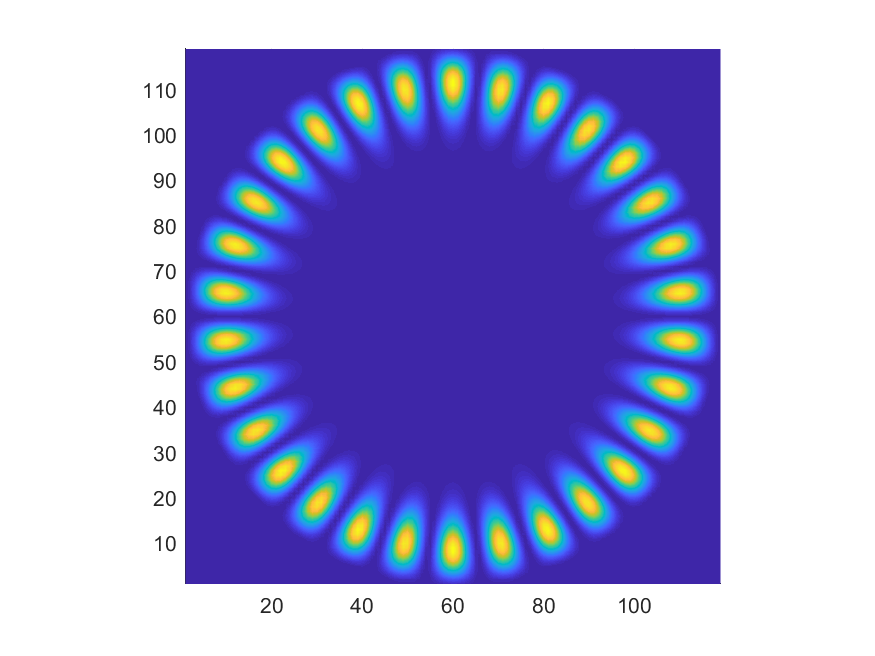
\includegraphics[width = 0.3\textwidth]{../images/figure/91_Psi.png}
        }
        \subfigure[$n=84(n \gg m)$]{
            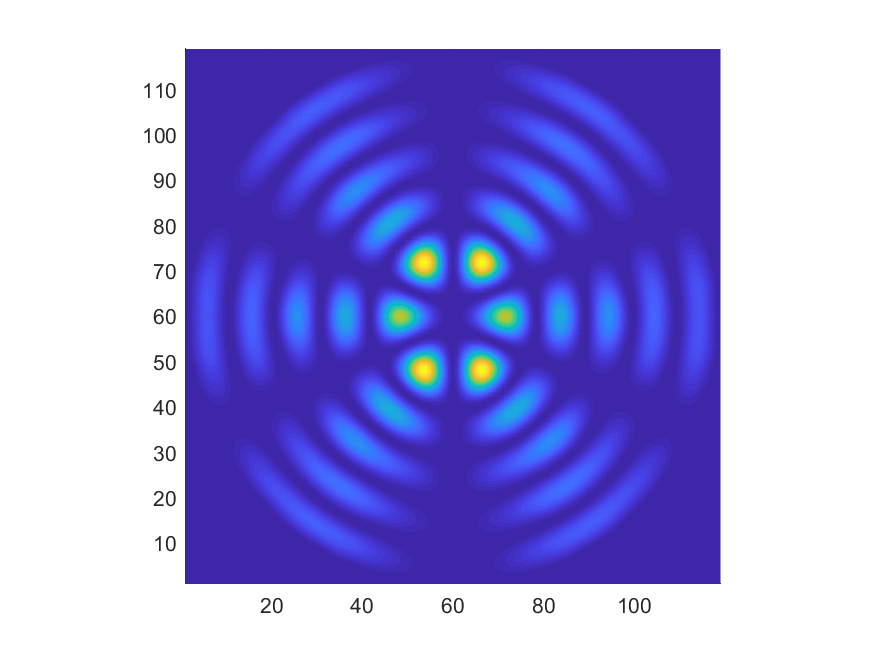
\includegraphics[width = 0.3\textwidth]{../images/figure/84_Psi.png}
        }
        \subfigure[$n=97(n\approx m)$]{
            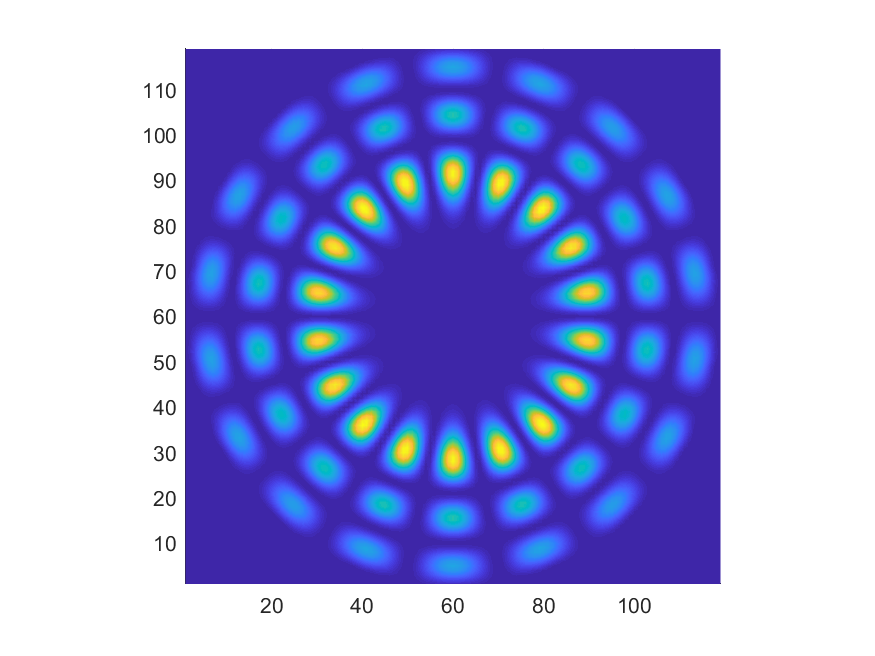
\includegraphics[width = 0.3\textwidth]{../images/figure/97_Psi.png}
        }
        \caption{波函数$\psi$的模方}
    \end{figure}
\end{frame}


\begin{frame}
    \frametitle{未处理的Husimi图}
    \begin{figure}
        \centering
        \subfigure[$n=91$]{
            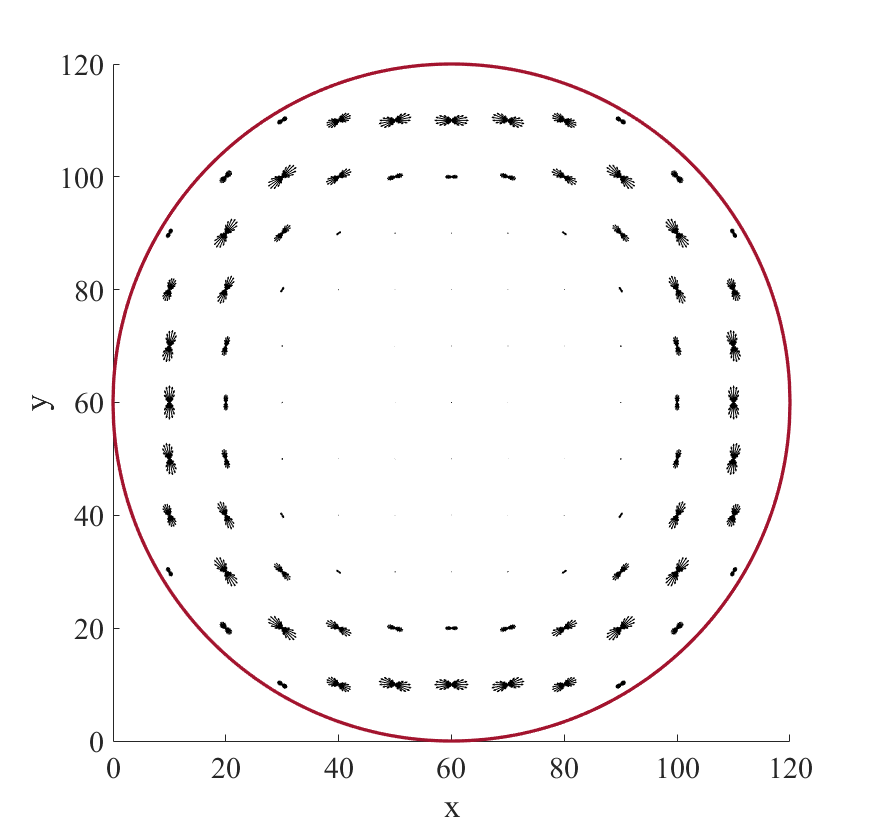
\includegraphics[width = 0.3\textwidth]{../images/figure/0.1_91_HusimiMap.png}
        }
        \subfigure[$n=84$]{
            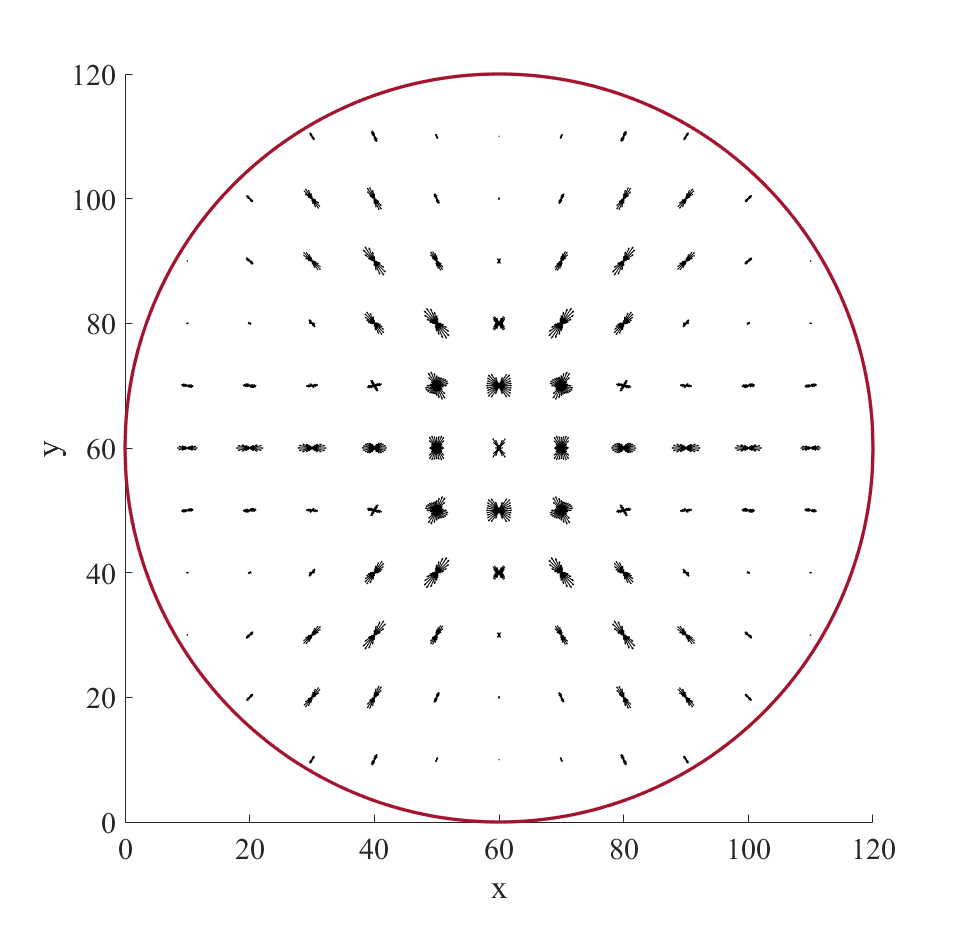
\includegraphics[width = 0.3\textwidth]{../images/figure/0.1_84_HusimiMap.png}
        }
        \subfigure[$n=97$]{
            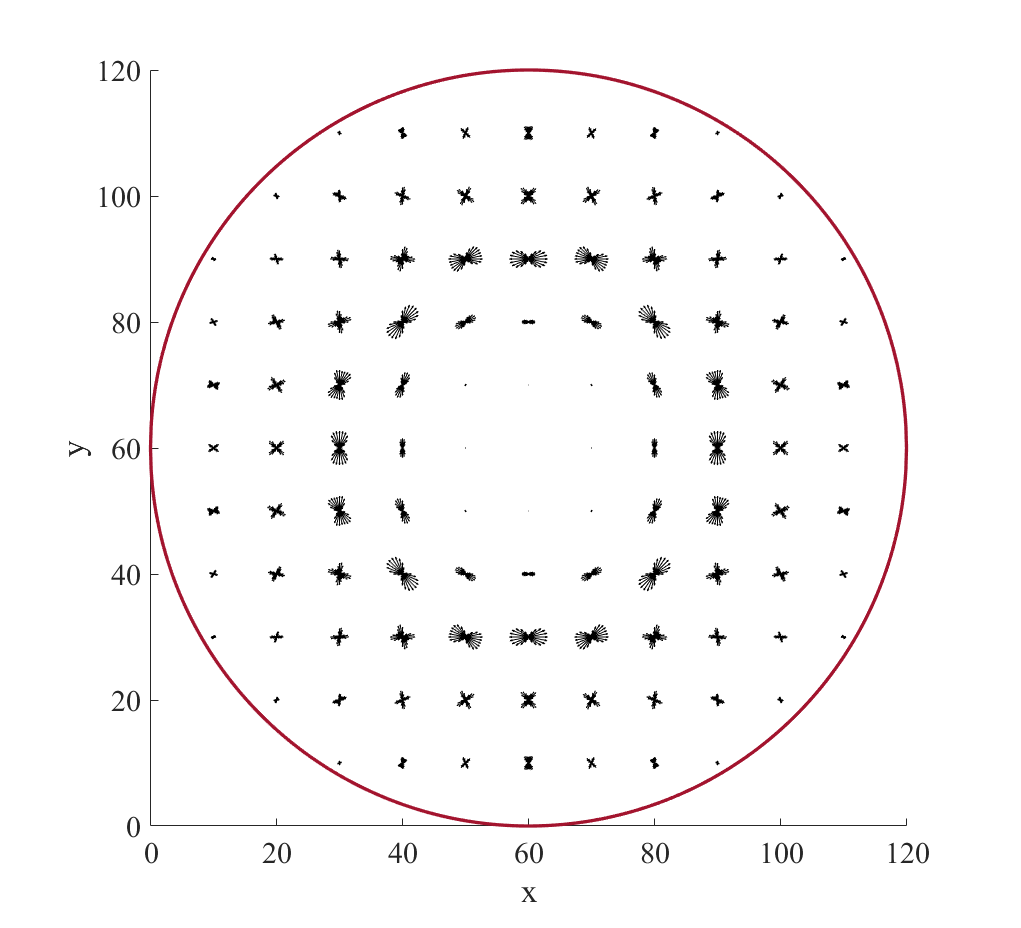
\includegraphics[width = 0.3\textwidth]{../images/figure/0.1_97_HusimiMap.png}
        }
        \caption{波函数$\psi$的Husimi图}
    \end{figure}
\end{frame}


\begin{frame}
    \frametitle{处理过的Husimi图}
    \begin{figure}
        \centering
        \subfigure[$n=91$]{
            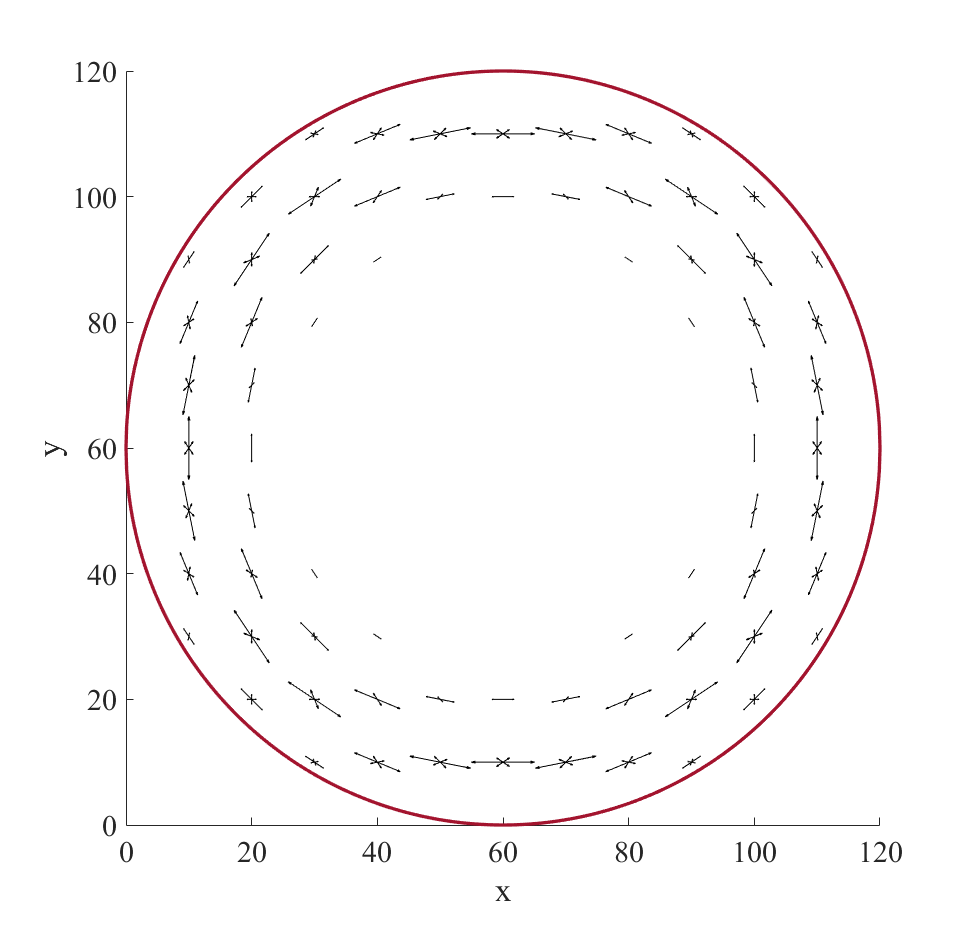
\includegraphics[width = 0.3\textwidth]{../images/figure/0.1_91_ProcHusimiMap.png}
        }
        \subfigure[$n=84$]{
            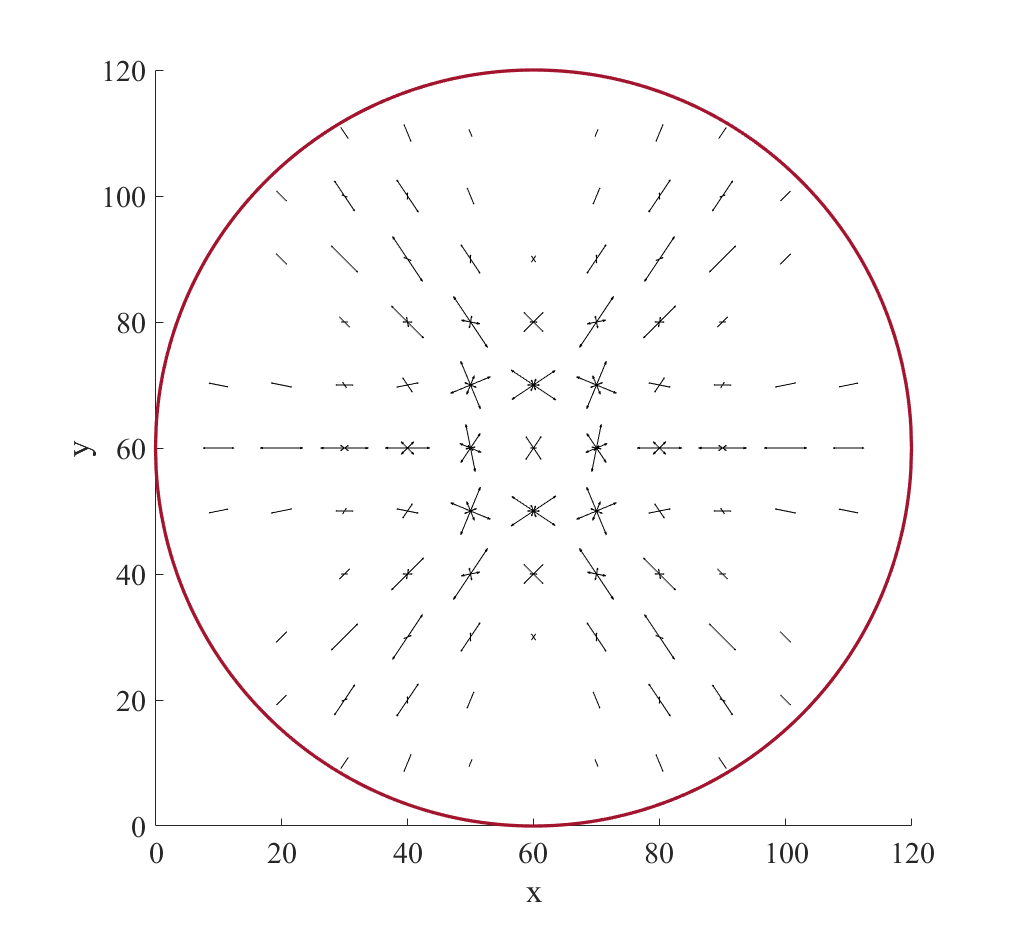
\includegraphics[width = 0.3\textwidth]{../images/figure/0.1_84_ProcHusimiMap.png}
        }
        \subfigure[$n=97$]{
            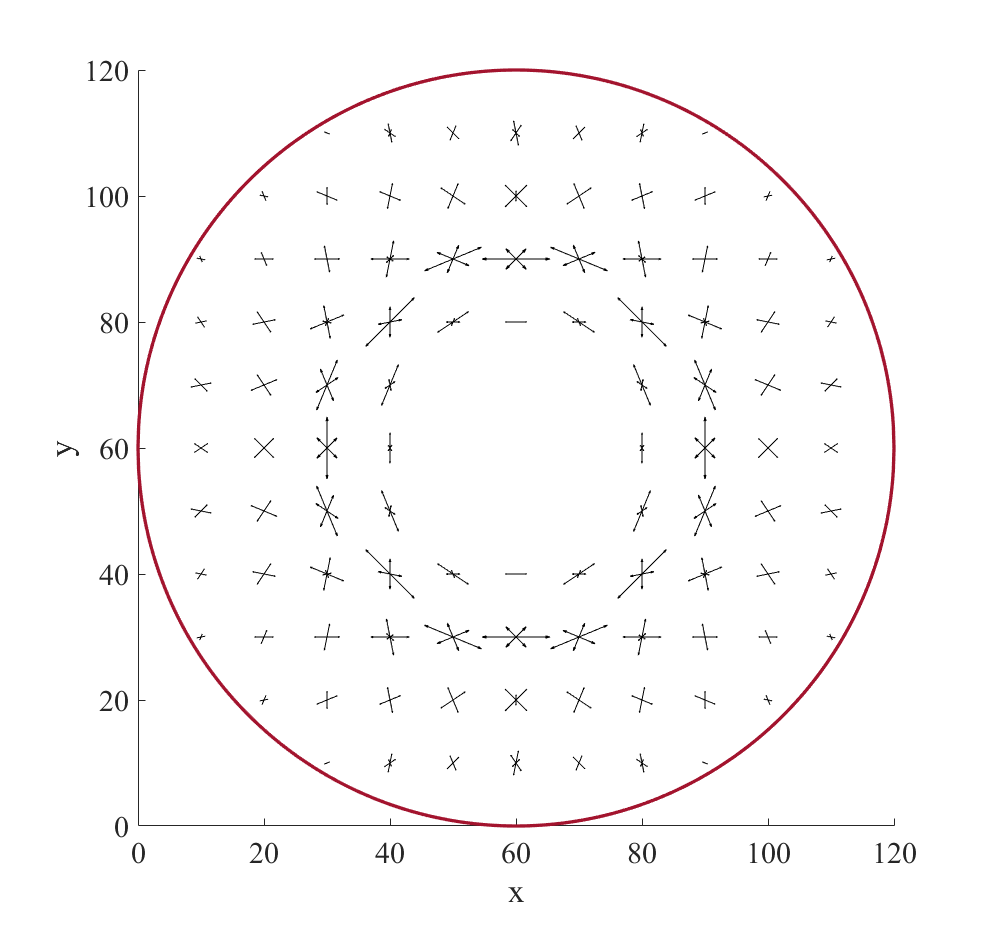
\includegraphics[width = 0.3\textwidth]{../images/figure/0.1_97_ProcHusimiMap.png}
        }
        \caption{波函数$\psi$处理过的Husimi图(MMA)。}
    \end{figure}
    上面的结果与文中\cite{mason2015revealing}图2:(a)-(e)的结果相似。
\end{frame}

\begin{frame}
    \frametitle{软墙($V=V_0(\mathbf{r})$)}
    \begin{figure}
        \centering
        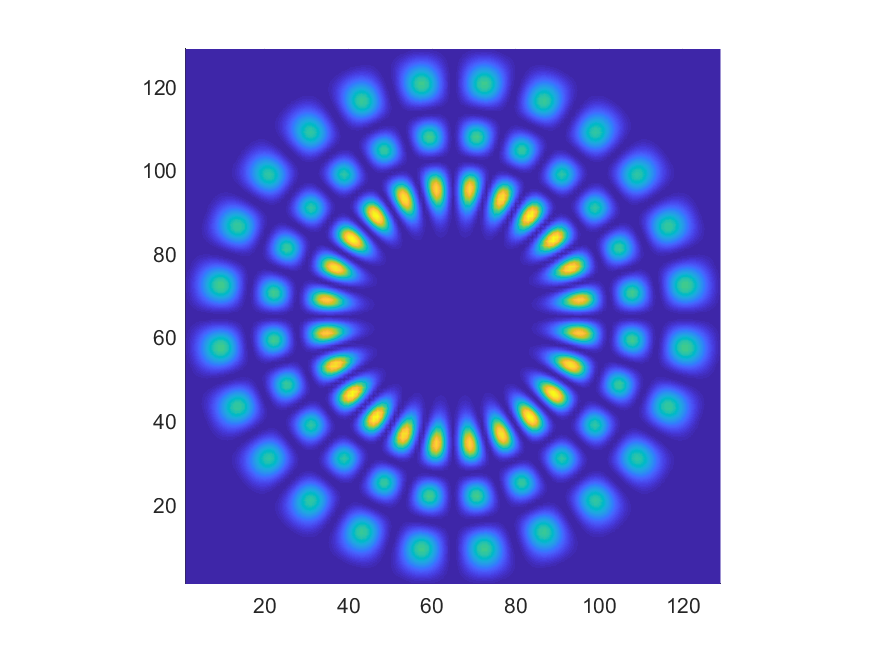
\includegraphics[width = 0.6\textwidth]{../images/figure/141_Psi.png}
        \caption{波函数$\psi$的模方,$n=141$}
    \end{figure} 
\end{frame}

\begin{frame}
    \frametitle{未处理的Husimi图}
    \begin{figure}
        \centering
        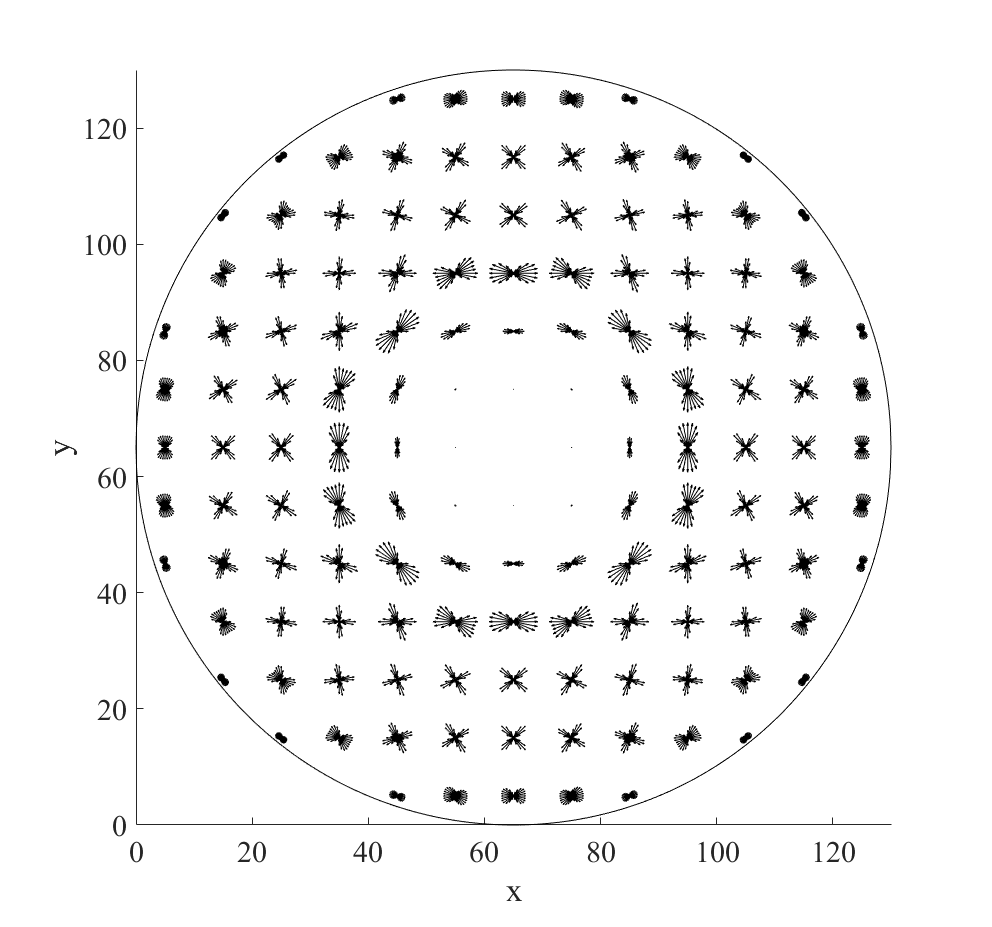
\includegraphics[width = 0.55\textwidth]{../images/figure/141_h_HusimiMap.png}
        \caption{Raw Husimi Map,$n=141$}
    \end{figure} 
\end{frame}

\begin{frame}
    \frametitle{处理过的Husimi图}
    \begin{figure}
        \centering
        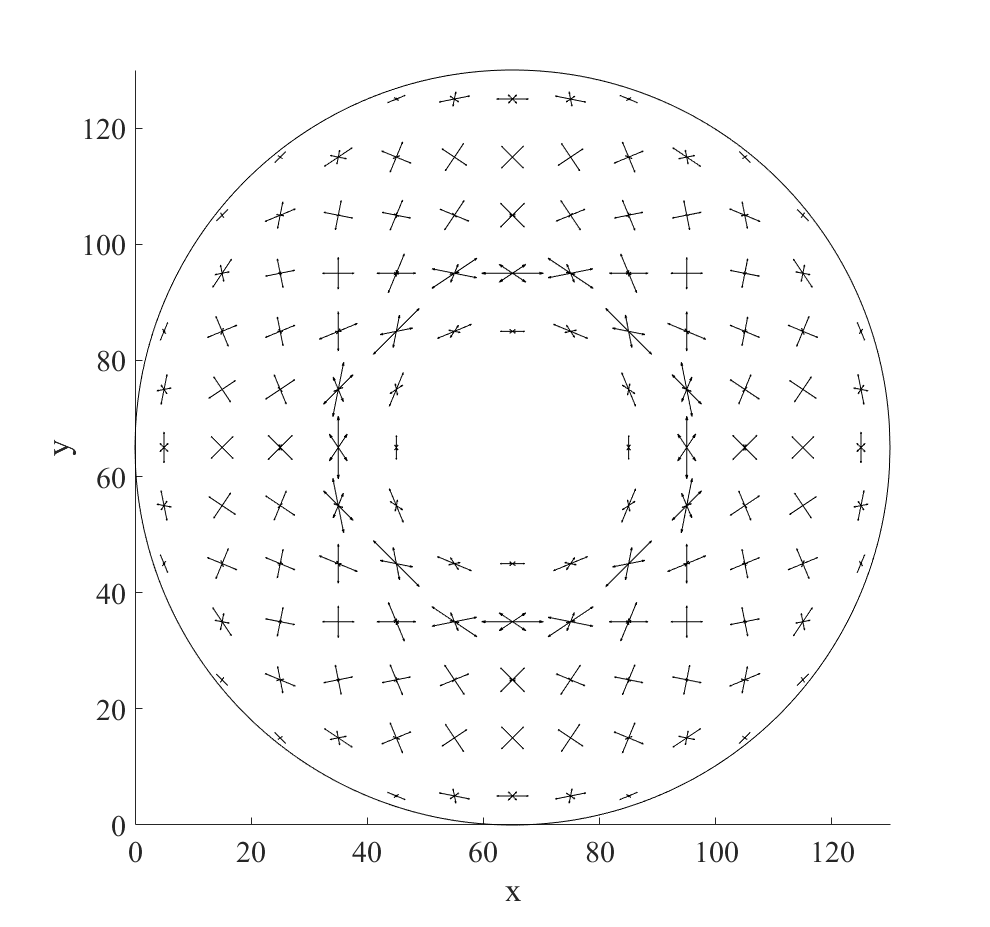
\includegraphics[width = 0.55\textwidth]{../images/figure/141_h_pHusimiMap.png}
        \caption{Processed Husimi Map,$n=141$}
    \end{figure} 
\end{frame}

\begin{frame}
    \frametitle{加入磁场}
    \begin{figure}
        \centering
        \subfigure[$n=188$]{
            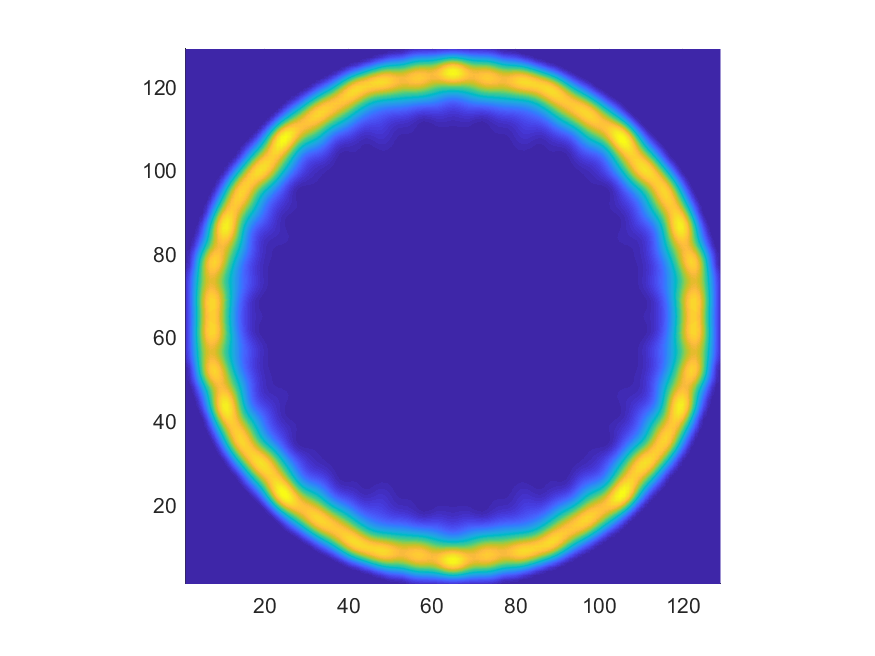
\includegraphics[width = 0.4\textwidth]{../images/figure/188_Psi.png}
        }
        \subfigure[$n=196$]{
            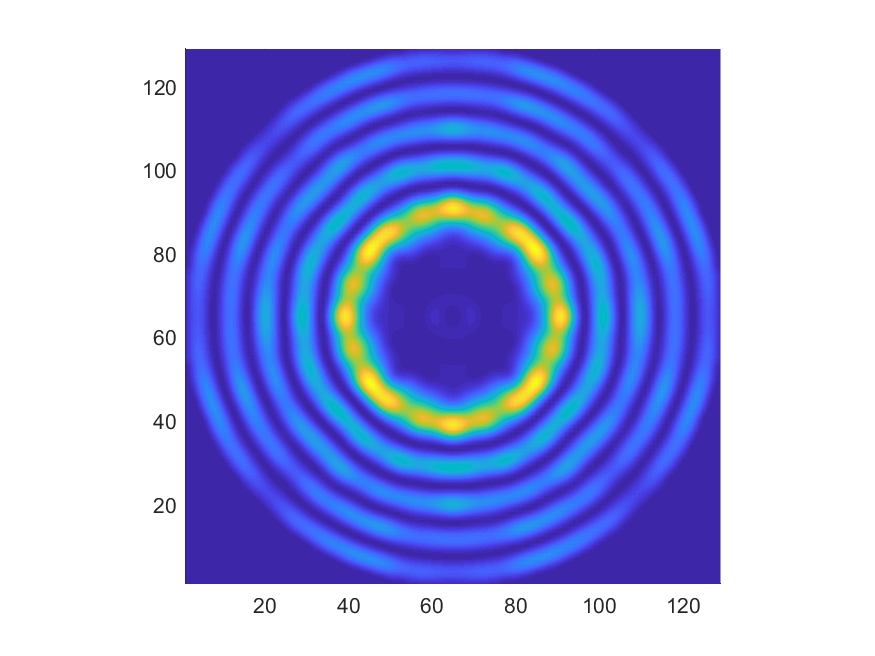
\includegraphics[width = 0.4\textwidth]{../images/figure/196_Psi.png}
        }
        \caption{波函数$\psi$的模方}
    \end{figure} 
\end{frame}

\begin{frame}
    \frametitle{加入磁场}
    \begin{figure}
        \centering
        \subfigure[$n=188$]{
            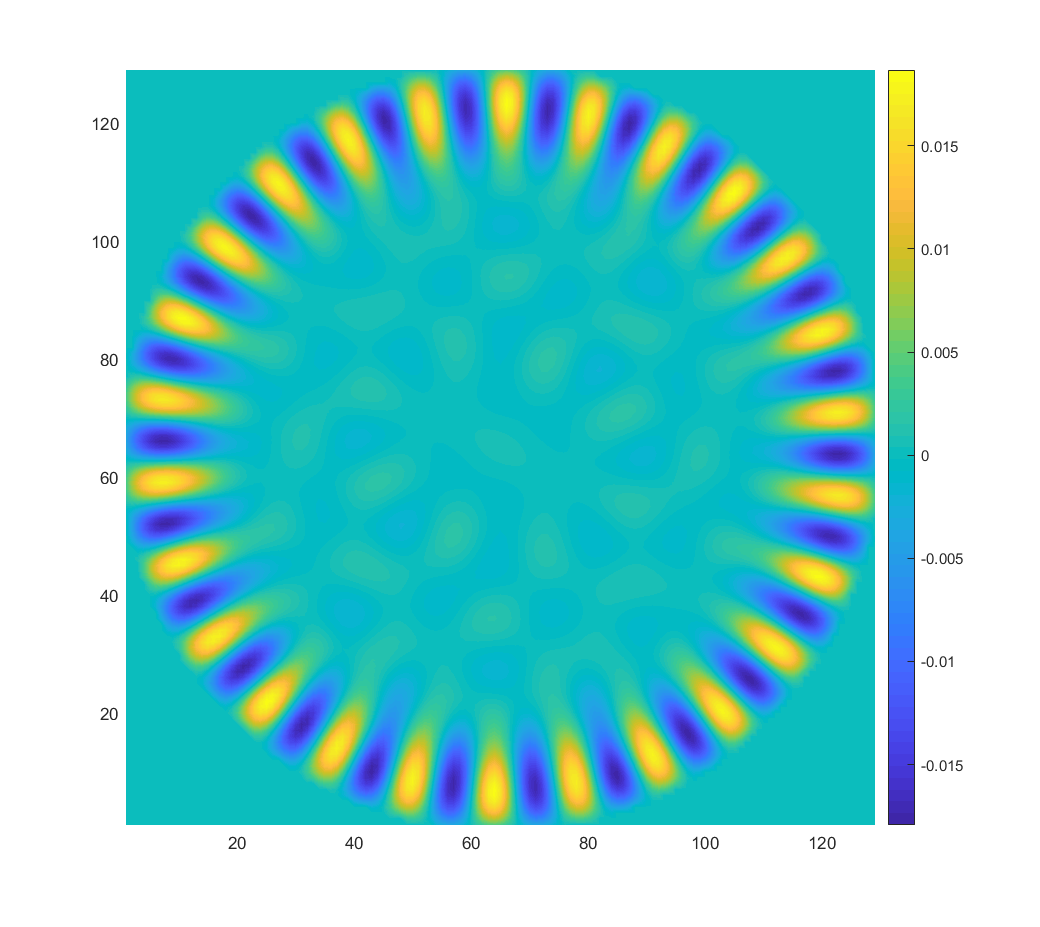
\includegraphics[width = 0.4\textwidth]{../images/figure/188_real.png}
        }
        \subfigure[$n=196$]{
            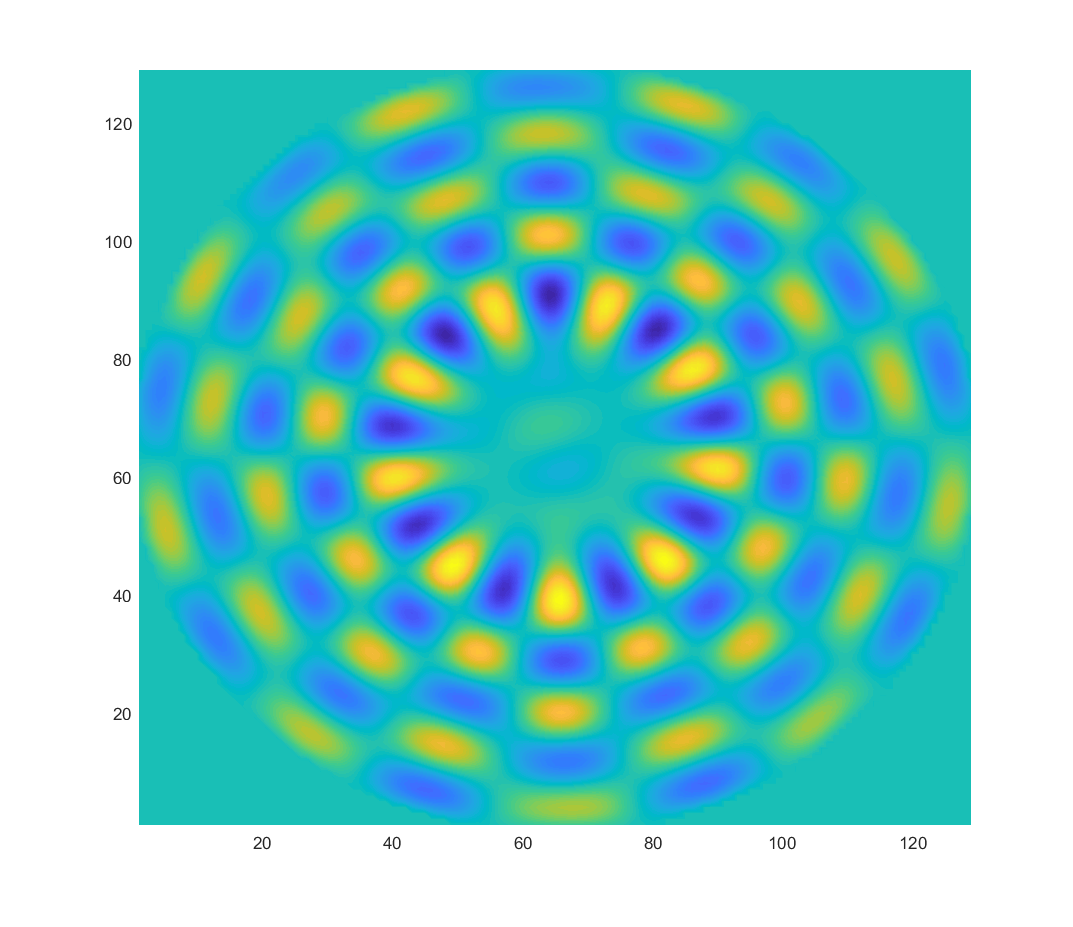
\includegraphics[width = 0.4\textwidth]{../images/figure/196_real.png}
        }
        \caption{波函数$\psi$的实部}
    \end{figure} 
\end{frame}

\begin{frame}
    \frametitle{未处理的Husimi图}
    \begin{figure}
        \centering
        \subfigure[$n=188$]{
            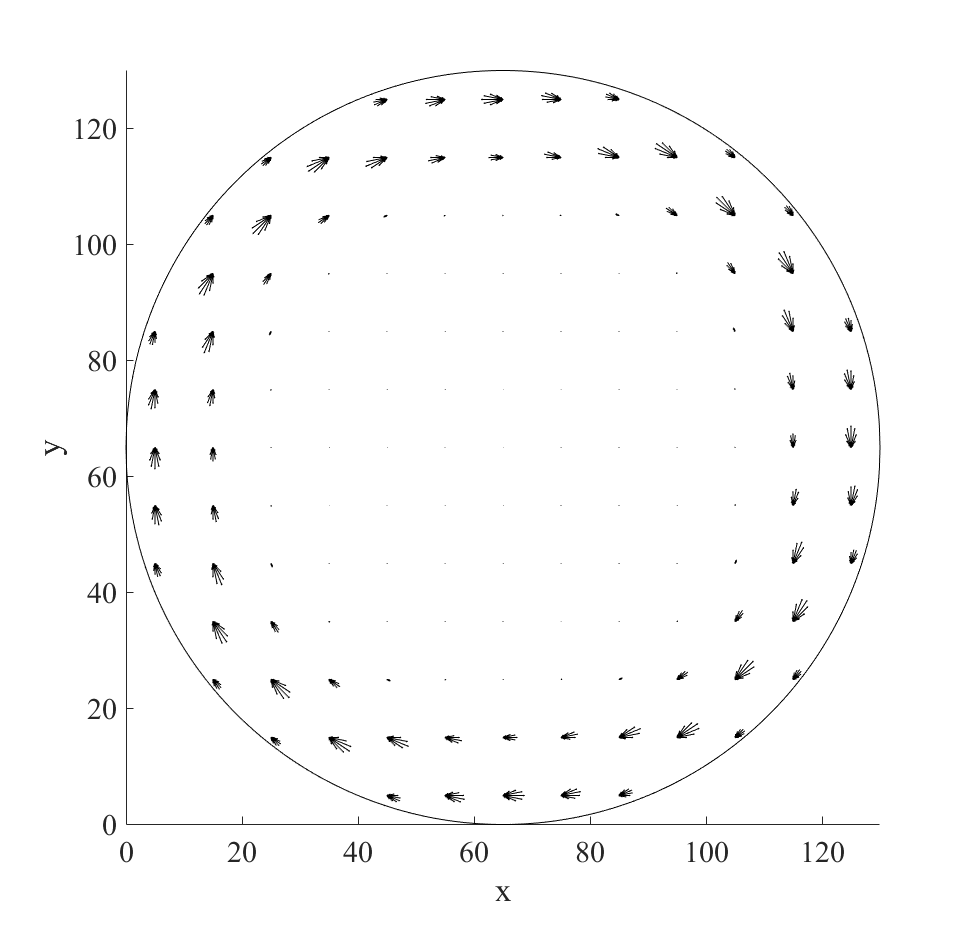
\includegraphics[width = 0.4\textwidth]{../images/figure/188_m_HusimiMap.png}
        }
        \subfigure[$n=196$]{
            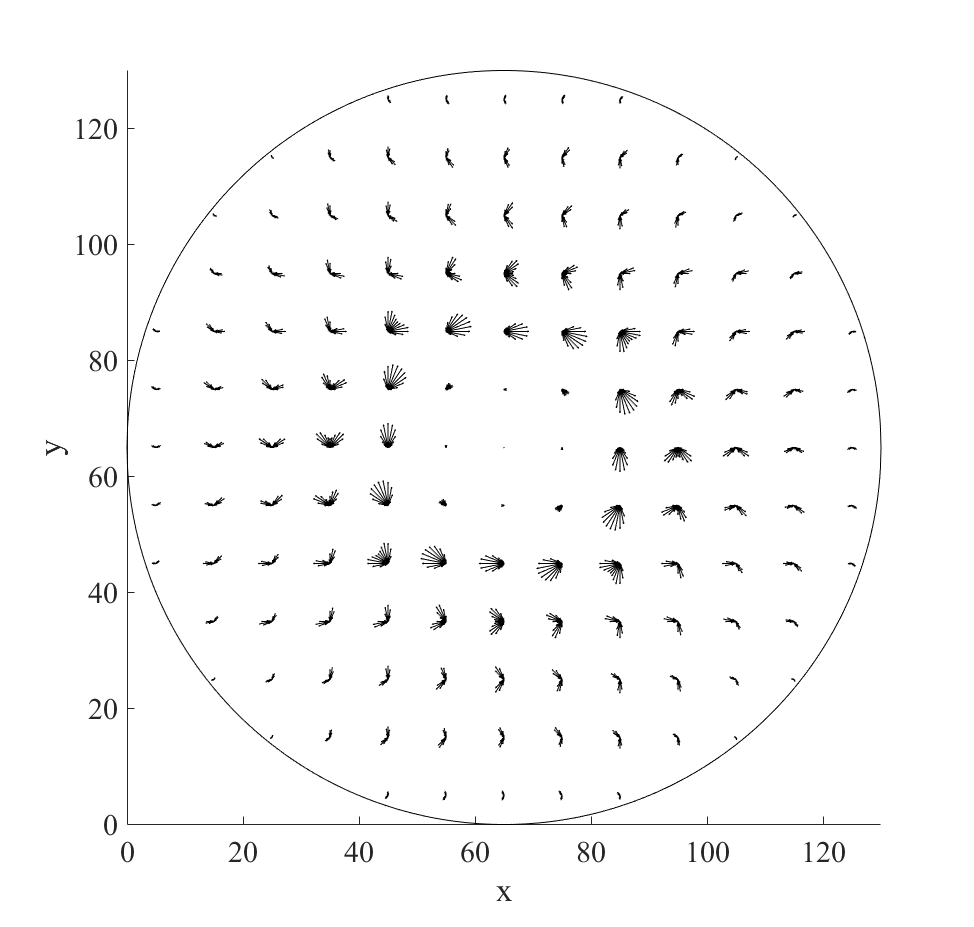
\includegraphics[width = 0.4\textwidth]{../images/figure/196_m_HusimiMap.png}
        }
        \caption{Raw Husimi Map}
    \end{figure}
\end{frame}

\begin{frame}
    \frametitle{处理过的Husimi图}
    \begin{figure}
        \centering
        \subfigure[$n=188$]{
            \includegraphics[width = 0.4\textwidth]{../images/figure/188_m_pHusimiMap.png}
        }
        \subfigure[$n=196$]{
            \includegraphics[width = 0.4\textwidth]{../images/figure/196_m_pHusimiMap.png}
        }
        \caption{Processed Husimi Map}
    \end{figure} 
\end{frame}

\subsection{运动场区域}

\begin{frame}
    \frametitle{采样点}

    \begin{figure}
        \centering
        \includegraphics[width = 0.8\textwidth]{../images/figure/stadium_mesh.png}
        \caption{红点:采样点,绿色:格点}
    \end{figure}

\end{frame}

\begin{frame}
    \frametitle{V型}
    \begin{figure}
        \centering
        \includegraphics[width = 0.74\textwidth]{../images/figure/182_s_psi.png}
        \caption{波函数模方}
    \end{figure}
\end{frame}

\begin{frame}
    \frametitle{V型}
    \begin{figure}
        \centering
        \includegraphics[width = 0.9\textwidth]{../images/figure/182_s_h.png}
        \caption{Raw Husimi Map}
    \end{figure}
\end{frame}

\begin{frame}
    \frametitle{V型}
    \begin{figure}
        \centering
        \includegraphics[width = 0.9\textwidth]{../images/figure/182_s_ph.png}
        \caption{Processed Husimi Map}
    \end{figure}
\end{frame}

\begin{frame}
    \frametitle{双三角型}
    \begin{figure}
        \centering
        \includegraphics[width = 0.74\textwidth]{../images/figure/74_s_psi.png}
        \caption{波函数模方}
    \end{figure}
\end{frame}

\begin{frame}
    \frametitle{双三角型}
    \begin{figure}
        \centering
        \includegraphics[width = 0.9\textwidth]{../images/figure/74_s_h.png}
        \caption{Raw Husimi Map}
    \end{figure}
\end{frame}

\begin{frame}
    \frametitle{双三角型}
    \begin{figure}
        \centering
        \includegraphics[width = 0.9\textwidth]{../images/figure/74_s_ph.png}
        \caption{Processed Husimi Map}
    \end{figure}
\end{frame}

\begin{frame}
    \frametitle{双菱形型}
    \begin{figure}
        \centering
        \includegraphics[width = 0.74\textwidth]{../images/figure/169_s_psi.png}
        \caption{波函数模方}
    \end{figure}
\end{frame}

\begin{frame}
    \frametitle{双菱形型}
    \begin{figure}
        \centering
        \includegraphics[width = 0.9\textwidth]{../images/figure/169_s_h.png}
        \caption{Raw Husimi Map}
    \end{figure}
\end{frame}

\begin{frame}
    \frametitle{双菱形型}
    \begin{figure}
        \centering
        \includegraphics[width = 0.9\textwidth]{../images/figure/169_s_ph.png}
        \caption{Processed Husimi Map}
    \end{figure}
\end{frame}

\section*{开源}
\begin{frame}
    \frametitle{源代码}
        https://github.com/Mr-Xinyuan/RepeatedHusimiFlow
\end{frame}

\begin{frame}
    \frametitle{参考文献}
    \bibliography{../bibliography/database.bib}
\end{frame}


\section*{致谢}
\begin{frame}
    \frametitle{致谢}
    \begin{center}
        \Huge 谢谢
    \end{center}
\end{frame}

\end{document}